\documentclass[a4paper, 12pt, titlepage, oneside]{article}
\usepackage[utf8]{inputenc}
\usepackage[czech]{babel}
\usepackage[total={17cm,25cm}, top=3cm, left=2cm, includefoot]{geometry}
\usepackage[T1]{fontenc}
\usepackage{amsmath}
\usepackage{amsfonts}
\usepackage{amssymb}

\usepackage{fancyhdr}
\usepackage{amsmath} % větší zlomyk pmocí \dfrac
\usepackage{graphicx} % vkládání obrázků
\usepackage{pdflscape} % stránka na šířku
\usepackage{float} % H aby bloky neuplavali
\usepackage{ctable} % horozontální čára s nastavitelnou šířkou a mezerami od okolí

\usepackage{pdfpages} % vložení pdf stránky

% balíšky pro hypertextové odkazy a hlavička dokumentu
\usepackage[bookmarksopen,plainpages=false,urlcolor=blue,bookmarks, pdfauthor={Jan Vykydal}, pdftitle={SDR - Software Defined Radio}, pdfsubject={software defined receiver for shortwave band}, pdfkeywords={SDR, software defined radio, receiver, filter, digitization, microcontroller, ATmega8, mixer, DDS, direct digital synthesis, oscillator, Johnson counter, quadrature detector.}]{hyperref}
\usepackage{url}

% náhledy stránek pro pdf
\usepackage{thumbpdf}






% záhlaví a zápatí ----------------------------------------------------------------
\pagestyle{fancy}
\fancyhf{}

% jednostranná sazba
%\fancyhead[R]{Jan \textsc{Vykydal} 4A}
\fancyhead[L]{SDR přijímač pro pásmo KV}
\fancyfoot[C]{\thepage/\pageref{konec}}
\renewcommand{\headrulewidth}{0.4pt}
\renewcommand{\footrulewidth}{0.4pt}

%\renewcommand{\figurename}{Obrázek č.}
%\renewcommand{\tablename}{Tabulka č.}

%\renewcommand{\contentsname}{Obsah} 
%\renewcommand{\listfigurename}{Seznam obrázků} 
%\renewcommand{\listtablename}{Seznam tabulek} 




\newcommand{\HRule}{\rule{\linewidth}{0.5mm}}

%odsazeni
\newcommand{\ind}{\hspace*{1cm}}

\setcounter{page}{1}


\begin{document}
 
	\begin{titlepage}
  \begin{center}

  % Upper part of the page. The '~' is needed because \\
  % only works if a paragraph has started.
  %
\includegraphics[width=0.15\textwidth]{./logo}~\\[1cm]

  \textsc{\LARGE Vyšší odborná škola a Střední průmyslová škola elektrotechnická Olomouc}%\\[1.5cm]

	% logo školy
	\begin{figure}[H]
    \centering
    
\includegraphics[width=4cm]{img/logo/logo.pdf}
  \end{figure}

  \textsc{\Large STŘEDOŠKOLSKÁ ODBORNÁ ČINNOST}\\[0.5cm]
  Obor 10. elektrotechnika, elektronika a telekomunikace\\[.2cm]
	
	
	
  % Title
  \HRule \\[0.4cm]
  { \huge \bfseries SDR přijímač pro pásmo KV\\[0.4cm] }

  \HRule \\[.5cm]
  
  SDR RECEIVER FOR SW BAND\\[1.5cm]
		
  % Author and supervisor
  \emph{Autor:} Jan \textsc{Vykydal}
  
  \vfill

  % Bottom of the page
  {\large \today}

  \end{center}
\end{titlepage}

	\clearpage
	\setcounter{page}{2}
	%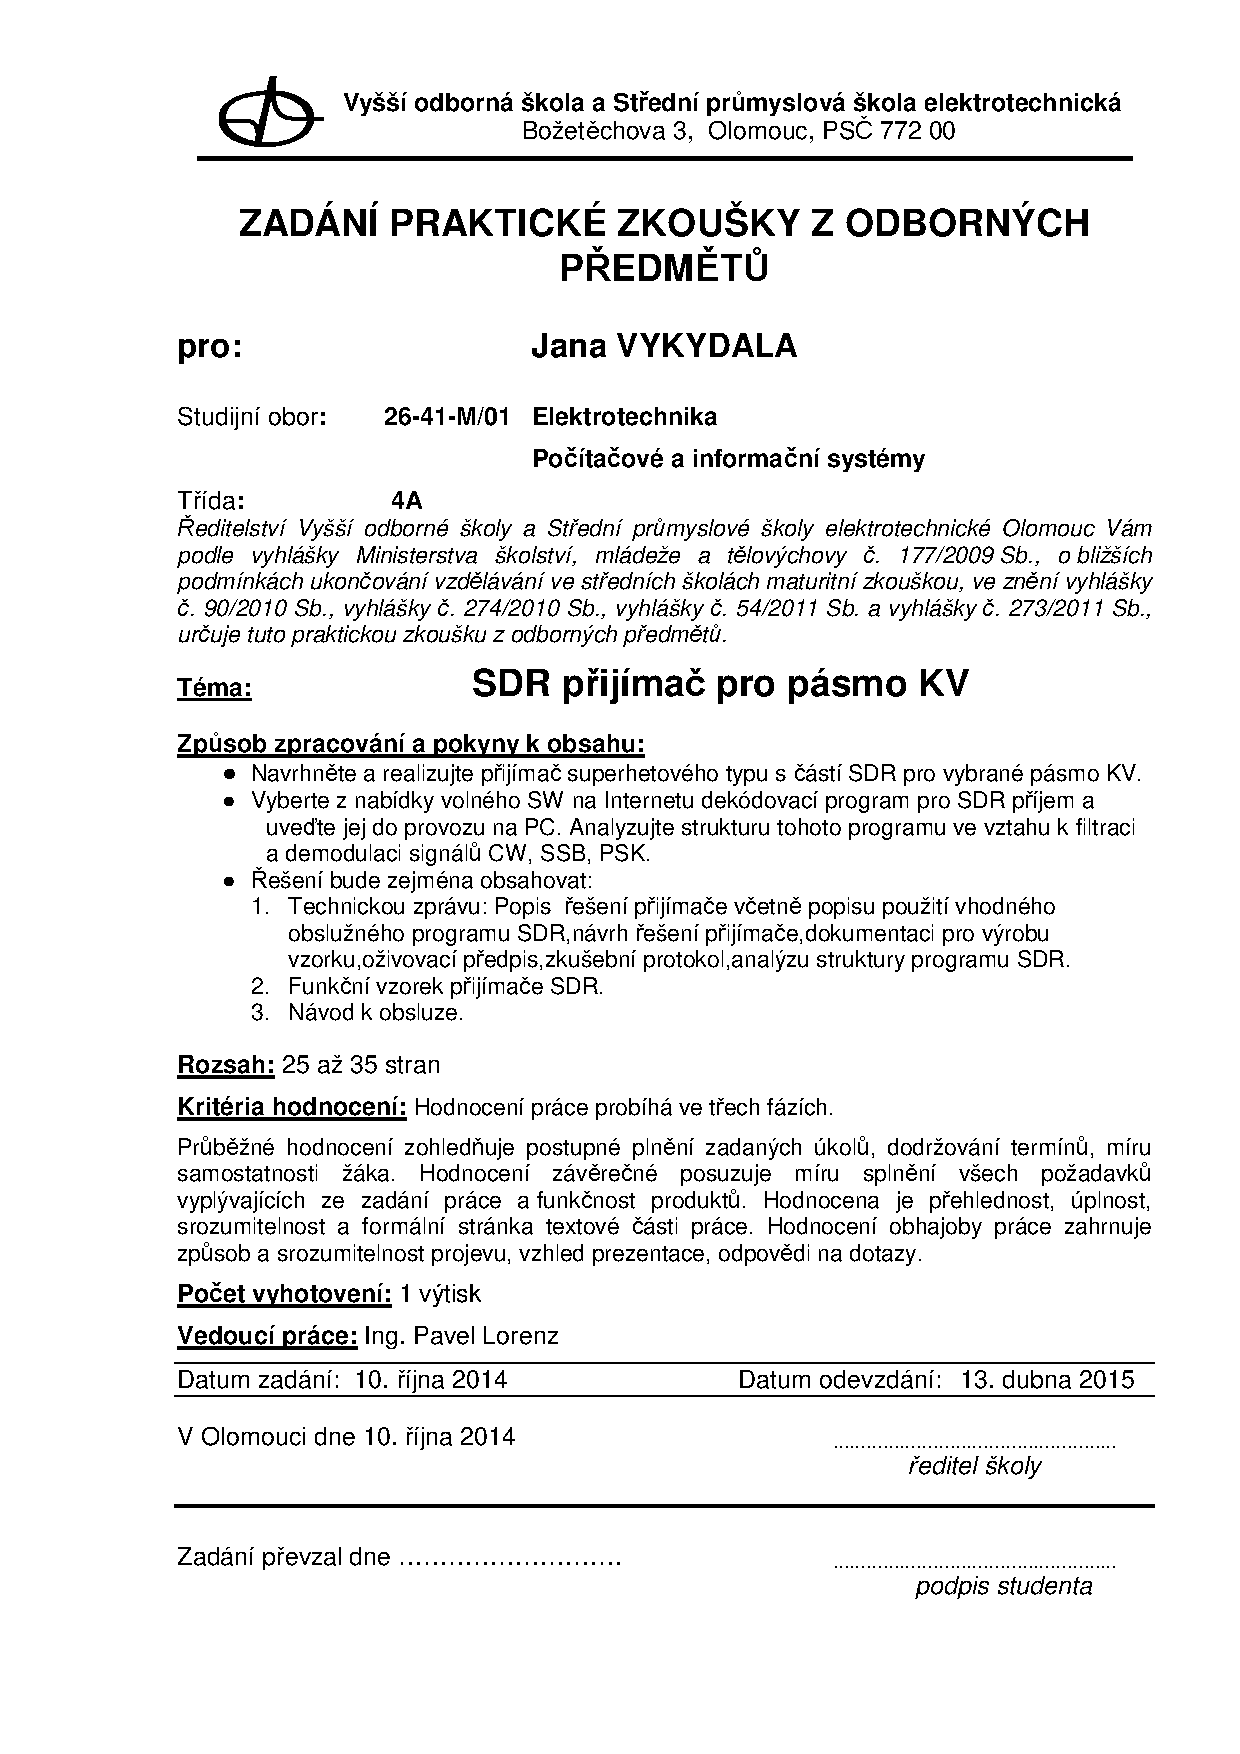
\includepdf[landscape=false]{zadani.pdf}	
	%\setcounter{page}{3}

\clearpage
\thispagestyle{empty}

Prohlašuji, že jsem praktickou zkoušku vypracoval samostatně a všechny prameny jsem uvedl v seznamu použité literatury.
\newline\newline
\begin{flushright}
	\begin{minipage}[H]{6cm}
		\begin{center}
			\dotfill\newline
			jméno a příjmení studenta
		\end{center}		
	\end{minipage}
\end{flushright}	

\vspace*{5cm}

Chtěl bych vyslovit poděkování panu Ing. Pavlu Lorenzovi, Ing. Jiřímu Burdovi a Ing. Petru Ďurišovi, za odborné konzultace a poskytnuté informace. Dále bych chtěl poděkovat Ing. Petru Ďurišovi za pomoc s výrobou desek plošných spojů. V neposlední řadě patří velký dík mému tátovi, který mi pomohl s ukotvením antény a výrobou krabičky.
\newline\newline
\begin{flushright}
	\begin{minipage}[H]{6cm}
		\begin{center}
			\dotfill\newline
			jméno a příjmení studenta
		\end{center}		
	\end{minipage}
\end{flushright}
	

\vspace*{5cm}
	
Prohlašuji, že nemám námitek proti půjčování nebo zveřejňování mé práce nebo její části se souhlasem školy.
\newline\newline
\begin{flushright}
	\begin{minipage}[H]{6cm}
		\begin{center}
			\dotfill\newline
			jméno a příjmení studenta
		\end{center}		
	\end{minipage}
\end{flushright}	
	
	
	


\clearpage

	\clearpage
\vspace*{\fill}
\section*{Prohlášení}
\indent\indent Prohlašuji, že jsem svou práci vypracoval samostatně a použil jsem pouze podklady (literaturu, projekty, SW atd.) uvedené v seznamu vloženém v práci.
		
Nemám závažný důvod proti zpřístupňování této práce v souladu se zákonem č. 121/2000 Sb., o právu autorském, o právech souvisejících s právem autorským a o změně některých zákonů (autorský zákon) v platném znění. 
	\newline\newline
	V Olomouci dne \today\hspace*{4cm}podpis: \dotfill\newline

\clearpage
\vspace*{\fill}	
\section*{Poděkování}
\indent\indent Chtěl bych vyslovit poděkování panu Ing. Pavlu Lorenzovi, Ing. Jiřímu Burdovi a Ing. Petru Ďurišovi, za odborné konzultace a poskytnuté informace. Dále bych chtěl poděkovat Ing. Petru Ďurišovi za pomoc s výrobou desek plošných spojů. V neposlední řadě patří velký dík mému tátovi, který mi pomohl s ukotvením antény a výrobou krabičky.

\clearpage
\section*{ANOTACE}
\indent\indent Tato práce popisuje návrh, konstrukci a realizace SDR přijímače pro pásmo krátkých vln. Dále se věnuje digitálnímu zpracování signálu. Postupně je v textu rozebraná cesta signálu od antény až k operátorovi radiové stanice. Cílem projektu bylo získání nových znalostí a zkušeností z oblasti zpracování signálu a radio elektroniky. Výsledkem projektu je funkční přijímač určený pro příjem radiových stanic na pásmech krátkých vln.
\newline\newline	
\noindent\textbf{Klíčová slova:}
SDR, softwarově definované rádio, přijímač, filtr, digitalizace, mikrokontrolér, ATmega8, směšovač, DDS, přímá digitální syntéza, oscilátor, Johnsonův čítač, kvadraturní detektor.

\section*{ANNOTATION}
\indent\indent This work describes a design, construction and realization SDR radio for short waves. Futher it presents digital processing of signal. Text deconstructs signal's path step by step from anthena to radio station operator. Goal of the project was gain of knowledge and experience from field of processing signal and radioelectronics. Project's result is functional dedicated for recieving radiostations in short-wave band.
\newline\newline
\noindent\textbf{Key words:}
SDR, software defined radio, receiver, filter, digitization, microcontroller, ATmega8, mixer, DDS, direct digital synthesis, oscillator, Johnson counter, quadrature detector.

\vspace*{\fill}
	

	\clearpage
	\tableofcontents	
	\clearpage
	\section*{Úvod}
\addcontentsline{toc}{section}{Úvod} 
\indent\indent Cílem mé práce bylo navrhnout a realizovat SDR přijímač pro pásmo krátkých vln. Toto téma spojuje mikroprocesorovou a číslicovou techniku s radioelektronikou, kterou jsem si chtěl osahat. V úvodu bych chtěl dále vysvětlit, co se skrývá za zkratkou SDR.

Zkratka SDR znamená Software Defined Radio (v překladu Softwarově Definované Rádio). Jedná se o další vývojovou etapu rádiových přijímačů a vysílačů. Klasická analogová rádia se postupně vyvíjela od jednoduchých krystalových přijímačů s přímým zesílením, přes přímosměšující tranzistorové přijímače až k velmi složitým přijímačům typu superheterodyn s možnostmi přepínání nejrůznějších demodulací a velkým rozsahem přijímaných pásem. Tyto přijímače ale začínaly být tak složité, že se k napěťovým signálům nesoucím informace při jejich zpracování přičítal šum jednotlivých bloků. Tento šum pak výrazně zhoršoval kvalitu přijímaného signálu. SDR je moderní technologie, která se snaží tyto nežádoucí vlivy hardwarových komponentů omezit. Ideální SDR přijímač se skládá jen z antény analogově digitálního převodníku a digitálního obvodu, který signál demoduluje. Díky tomu se k přijímané informaci přidává jen minimální chyba při digitalizaci signálu. Tato technologie tedy posouvá zařízení pro rádiový přenos o světelné roky dál, jelikož je s jejich pomocí možné přenášet v podstatě libovolně modulovaný signál, a tím pak přenášet komprimované informace, nebo vytvářet nové digitální modulace. Obrovskou výhodou SDR přijímačů a vysílačů je jejich neustálé vylepšování bez nutnosti jakkoliv měnit hardware přijímače.
\begin{figure}[H]
	\centering
	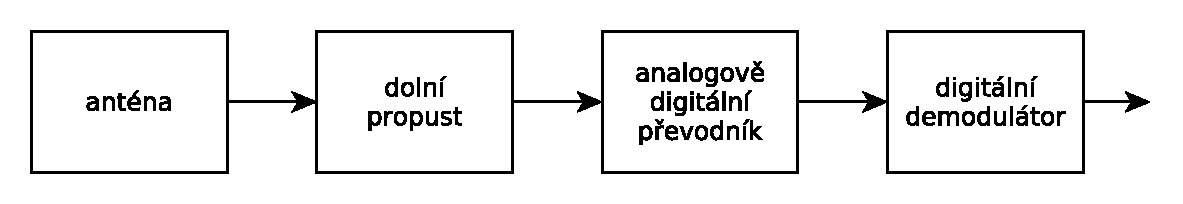
\includegraphics[width=170mm]{img/i_sdr.pdf}
	\caption{blokové schéma ideálního SDR přijímače}    		
\end{figure}

\clearpage
		
	
  		
  		
	\section{Koncepce přijímače}
\indent\indent V úvodu bylo uvedeno blokové zapojení ideálního SDR přijímače. Toto zapojení je ale náročné na realizaci, protože vstupní analogově digitální převodník  by musel mít vzorkovací frekvenci minimálně dle Shannonův-Nyquistův-Kotělnikova teorému $f_v > 2f_{max}$. Tedy pro přijímač určený k příjmu pásma 20 metrů by muselo pro vzorkovací frekvenci platit $f_v > 2 \cdot 14,35~MHz$. Takovéto převodníky se sice vyrábějí, ale jejich cena je nad rámec rozpočtu tohoto projektu. Dalším problémem by bylo zpracování objemného datového toku z těchto převodníků. Proto byl  tento koncept analogově digitálního převodníku přímo za anténou zamítnut. Namísto toho byla navržena taková koncepce, která umožňuje výstupní napěťový signál z SDR vzorkovat na prakticky libovolné zvukové kartě s linkovým vstupem.
\begin{figure}[H]
	\centering
	\label{obr:bs_sdr}
	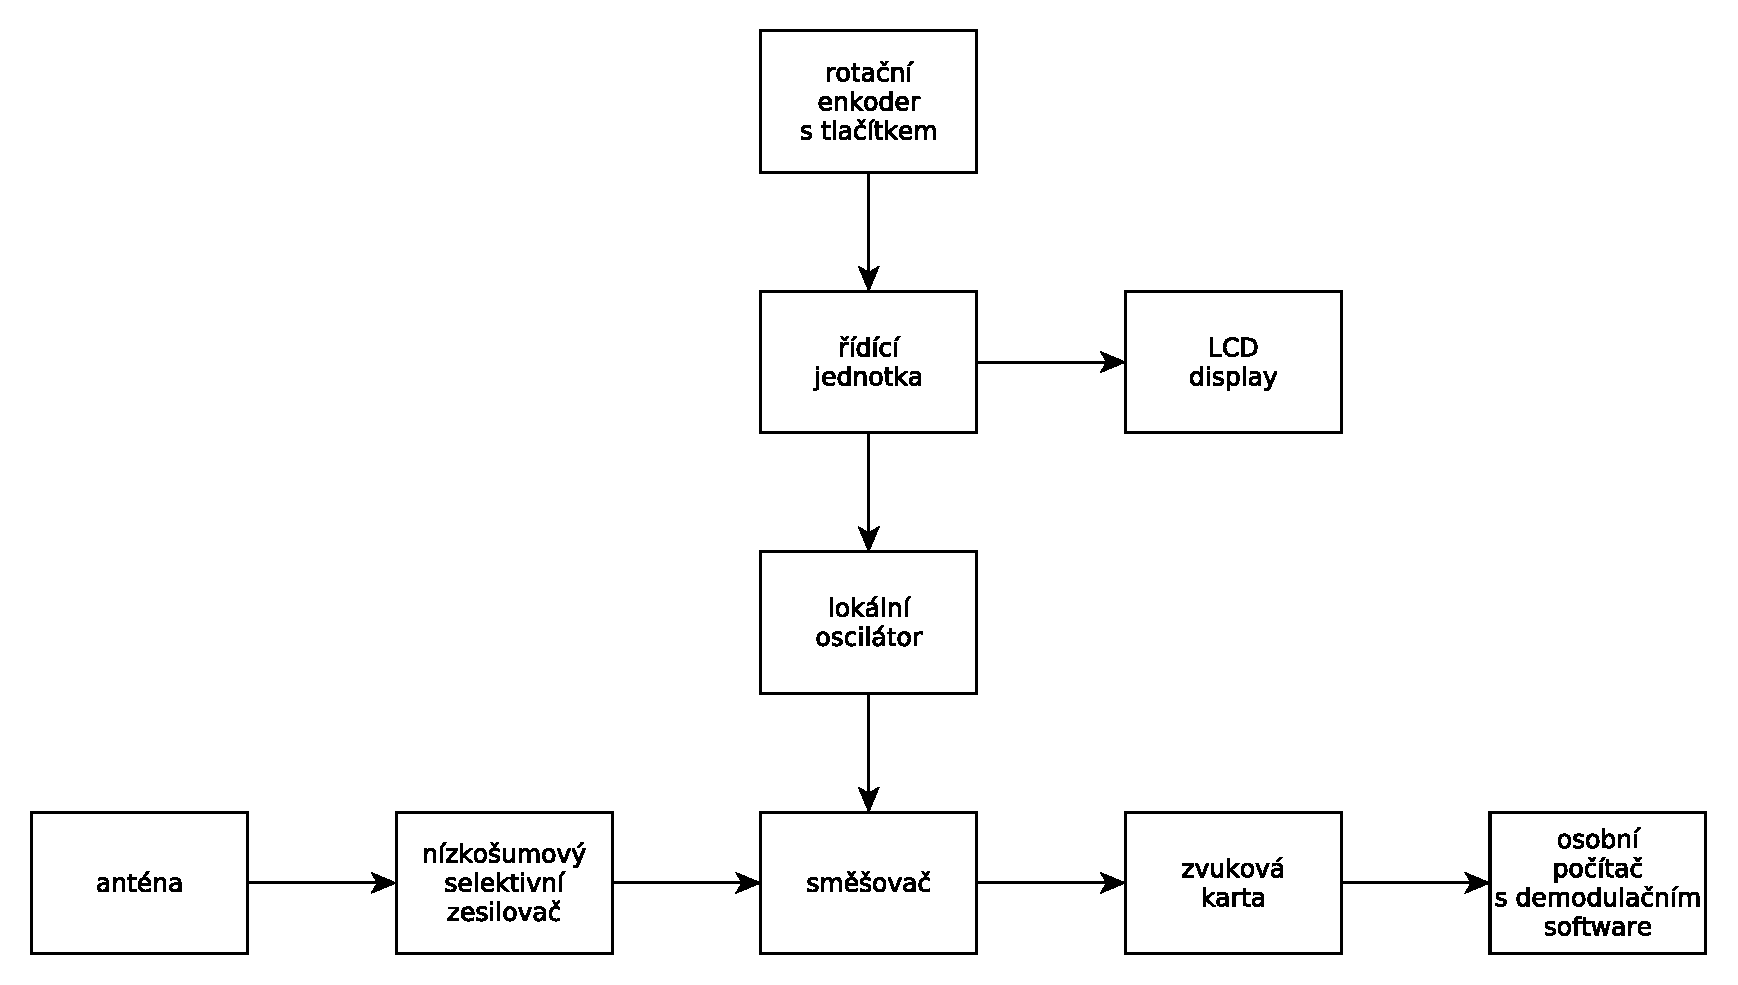
\includegraphics[width=170mm]{img/bs_sdr.pdf}
	\caption{blokové schéma navrženého přijímače}    		
\end{figure}

Toto blokové schéma představuje jednotlivé desky plošných spojů nebo jiných samostatných částí. Tyto bloky budou v následujícím textu postupně rozebírány.





\clearpage
	\clearpage
\section{Nízkošumový selektivní zesilovač}
%\subsection{Popis funkce obvodu}
\indent\indent Tento obvod má za úkol zesílit vstupní signál a současně odstranit nežádoucí signál mimo přijímané pásmo. Vstupní signál z antény je přiváděn konektorem P1, dále pokračuje k transformátoru T1. Ten slouží jako impedanční přizpůsobení, kdy upravuje  impedanci ze vstupních $50~\Omega$ směrem nahoru až na několik set ohmů. Impedance závisí na kmitočtu vstupního signálu. Sekundární vinutí transformátoru T1 tvoří s kondenzátorem C2 a kapacitním trimrem C3 paralelní rezonanční obvod naladěný na frekvenci $14~MHz$. Tento rezonanční obvod je spojen kapacitní vazbou, kterou tvoří kondenzátor C4 s dalším paralelním rezonančním obvodem. Ten je tvořen kondenzátorem C5, kapacitním trimrem C6 a primárním vinutím transformátoru T2. Tento rezonanční obvod je naladěný na frekvenci $14,35~MHz$. Další funkce transformátoru T2 je transformace impedance zpátky na $50~\Omega$. Transformátory T1 a T2 jsou navinuty na toroidním jádru Amidon T44-2. Upravený signál pokračuje dále přes vazební kondenzátor do tranzistorového zesilovače. Jedná se o zesilovač pracující ve třídě A a je postavený s tranzistorem KF630D. Teplotní stabilizaci zajišťuje záporná proudová zpětná vazba tvořená rezistory R3 a R4. Napětí báze je stabilizováno  zápornou napěťovou zpětnou vazbou tvořenou rezistory R1, R2 a R5. Výstupní proud z tranzistoru teče do bifilárně navinutého transformátoru T3. T3 tvoří sedm závitů izolovanou dvoulinkou drátu průměru $0,8~mm$ na toroidní jádro z materiálu N2. Tento transformátor přizpůsobuje výstupní impedanci na $50~\Omega$. Před výstupním konektorem je ještě zařazen kondenzátor C11, který slouží k oddělení stejnosměrné složky. Celý obvod se tedy chová jako aktivní frekvenční propust.

%\subsection{Frekvenční propust}
%\indent\indent 
%Jak již bylo zmíněno výše, jedná se o dva paralelní rezonanční obvody. Jeden je naladěný na $14.00~MHz$ a druhý na $14.35~MHz$, což odpovídá šířce přijímaného pásma. Transformátory jsou navinuty na toroidní jádra materiálu Amidon T-44-2. Oba transformátory jsou navinuty stejně. Rezonanční cívku tvoří 27 závitů měděným drátkem průměru $0.3~mm$. $50~\Omega$ výstup je navinut třemi závity měděného drátu průměru $0.8~mm$.

% selektivita
\begin{figure}[H]
	\centering
	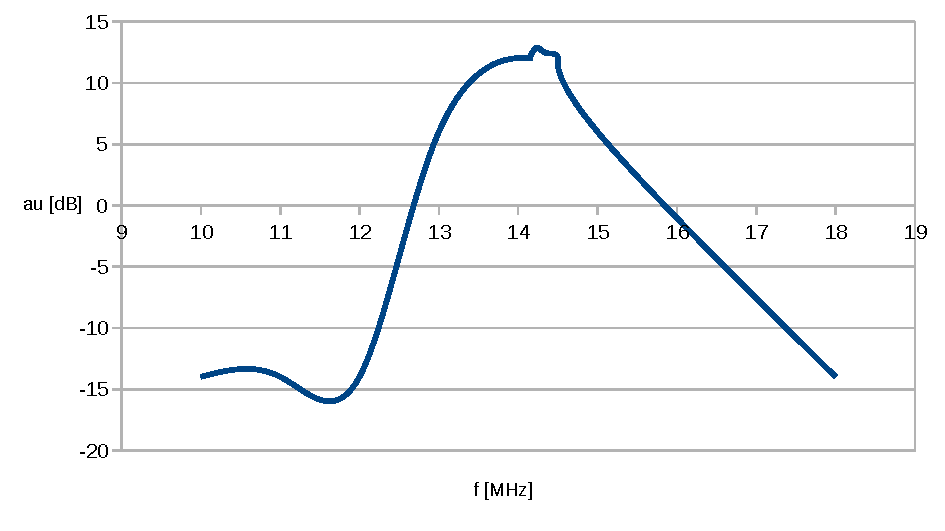
\includegraphics[width=170mm]{img/LNA/sel.pdf}
	\caption{Graf selektivnosti aktivní pásmové propusti}    		
\end{figure}

% schéma
\begin{landscape}
	\begin{figure}[h]
		\centering 	
		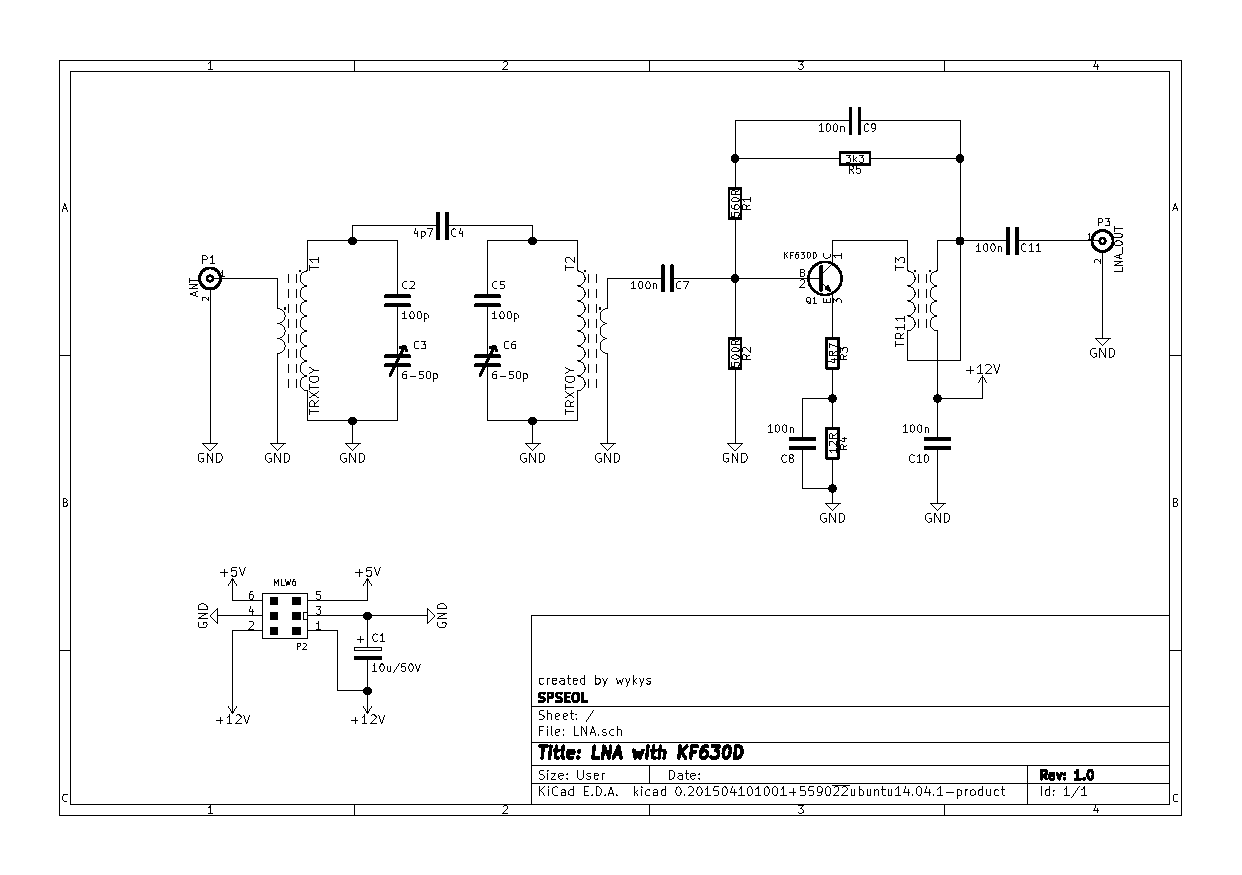
\includegraphics[height=\textwidth]{img/LNA/sch.pdf}
		\caption{Schéma zapojení nízkošumového selektivního zesilovače}	
	\end{figure}
\end{landscape}
%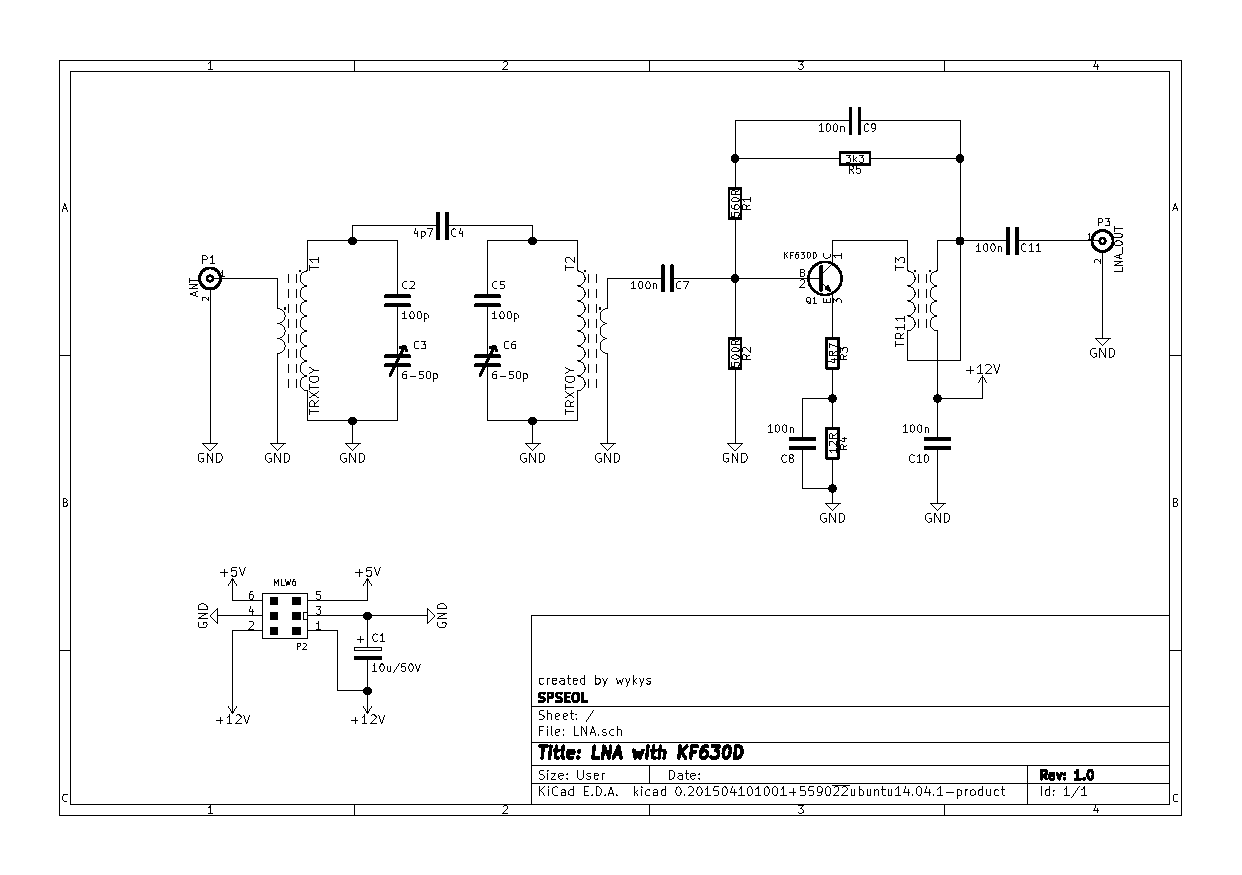
\includepdf[landscape=true]{img/LNA/sch.pdf}



%\subsection{Deska plošných spojů selektivního zesilovače}
%\indent\indent
%Desky plošných spojů jsou oboustranné.
Deska plošného spoje je zhotovena na oboustranném materiálu FR4. Spodní strana tvoří vlastní vrstvu spojů a na horní straně je rozlitá měď kvůli stínění obvodu.

% DPS
\begin{figure}[H]
	\centering
	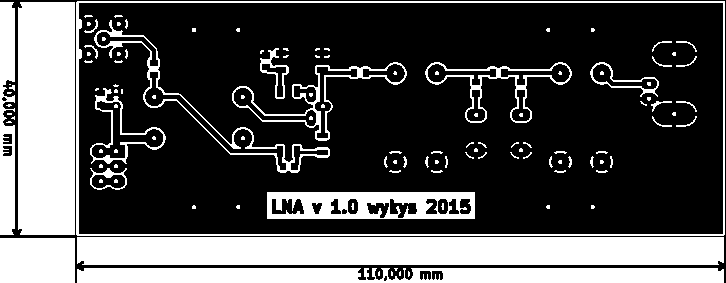
\includegraphics[width=170mm]{img/LNA/cu_b.pdf}
	\caption{Deska plošného spoje selektivního zesilovače, strana spojů}    		
\end{figure}

% os f
\begin{figure}[H]
	\centering
	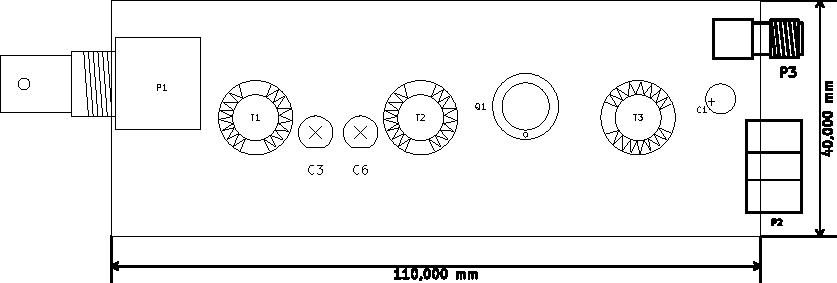
\includegraphics[width=170mm]{img/LNA/os_f.pdf}
	\caption{Osazovací plán selektivního zesilovače, strana součástek}    		
\end{figure}

% os b
\begin{figure}[H]
	\centering
	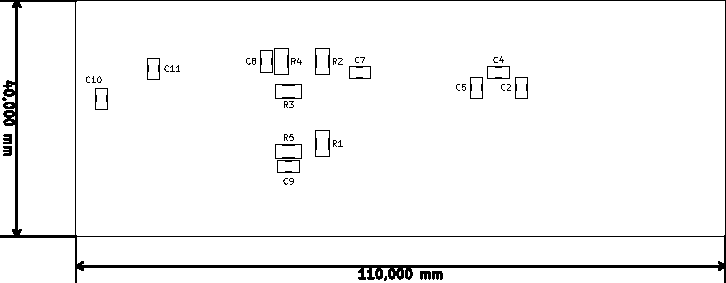
\includegraphics[width=170mm]{img/LNA/os_b.pdf}
	\caption{Osazovací plán selektivního zesilovače, strana spojů}    		
\end{figure}

\begin{table}[H]
	\begin{center}
		\caption{Tabulka použitých součástek pro desku selektivního zesilovače}
		\label{tab:lna_os} 
		\begin{tabular}[H]{!{\vrule width 1pt}c|c|c|c!{\vrule width 1pt}}
		    \specialrule{1pt}{0pt}{0pt} 
		    \textbf{Určovatel}	&	\textbf{Pouzdro}	&	\textbf{Množství}	&	\textbf{Určení}	\\\specialrule{1pt}{0pt}{0pt} 
			T3	&	N2	&	1	&	TR11	\\\hline
			T1,T2	&	Amidon-T44-2	&	2	&	TRXTOY	\\\hline
			C1	&	Elko\_vert\_11x5mm\_RM2.5	&	1	&	10u/50v	\\\hline
			C2,C5	&	C\_0805	&	2	&	100p	\\\hline
			C3,C6	&	CT	&	2	&	6-50p	\\\hline
			C4	&	C\_0805	&	1	&	4p7	\\\hline
			C7,C8,C9,C10,C11	&	C\_0805	&	5	&	100n	\\\hline
			P1	&	BNC&	1	&	ANT	\\\hline
			P2	&	MLW6	&	1	&	napájení	\\\hline
			P3	&	MCX	&	1	&	LNA\_OUT	\\\hline
			Q1	&	TO5	&	1	&	KF630D	\\\hline
			R1	&	R\_1206	&	1	&	560R	\\\hline
			R2	&	R\_1206	&	1	&	500R	\\\hline
			R3	&	R\_1206	&	1	&	4R7	\\\hline
			R4	&	R\_1206	&	1	&	12R	\\\hline
			R5	&	R\_1206	&	1	&	3k3	\\\hline
			M1,M2,M3,M4	&	M3	&	4	&	M3	\\\specialrule{1pt}{0pt}{0pt} 
		\end{tabular}		     
	\end{center}
\end{table}
	
	\clearpage
\section{Řídící jednotka}
\indent\indent Tento modul slouží k ovládání celého rádia, nastavení a zobrazení přijímané frekvence a dále k řízení generátoru DDS pro ovládání výstupního kmitočtu lokálního oscilátoru.

Řídící jednotka je postavena na jednočipovém mikrokontroléru ATmega8, taktovaného na $11,0592~MHz$. Frekvence hodin není náhodná, ale je vybrána záměrně, jelikož díky této taktovací frekvenci může mikrokontrolér komunikovat s okolím pomocí rozhraní USART rychlostí $9600~Bdps$. K mikrokontroléru je připojen znakový LCD displej RC1602B2-BIW-CSX s řadičem HD44780. Jedná se o displej, který zobrazuje informaci ve dvou řádcích, každý po 16 znacích. Displej je použit k zobrazování frekvence přijímané stanice a velikosti ladícího kroku. Dále je k mikrokontroléru připojen rotační enkodér s vestavěným tlačítkem. Pro změnu frekvence nebo velikosti ladícího kroku. Na základě údajů získaných od operátora řídící jednotka nakonfiguruje DDS obvod v lokálním oscilátoru.


% vyvojak A
\begin{figure}[H]
	\centering
	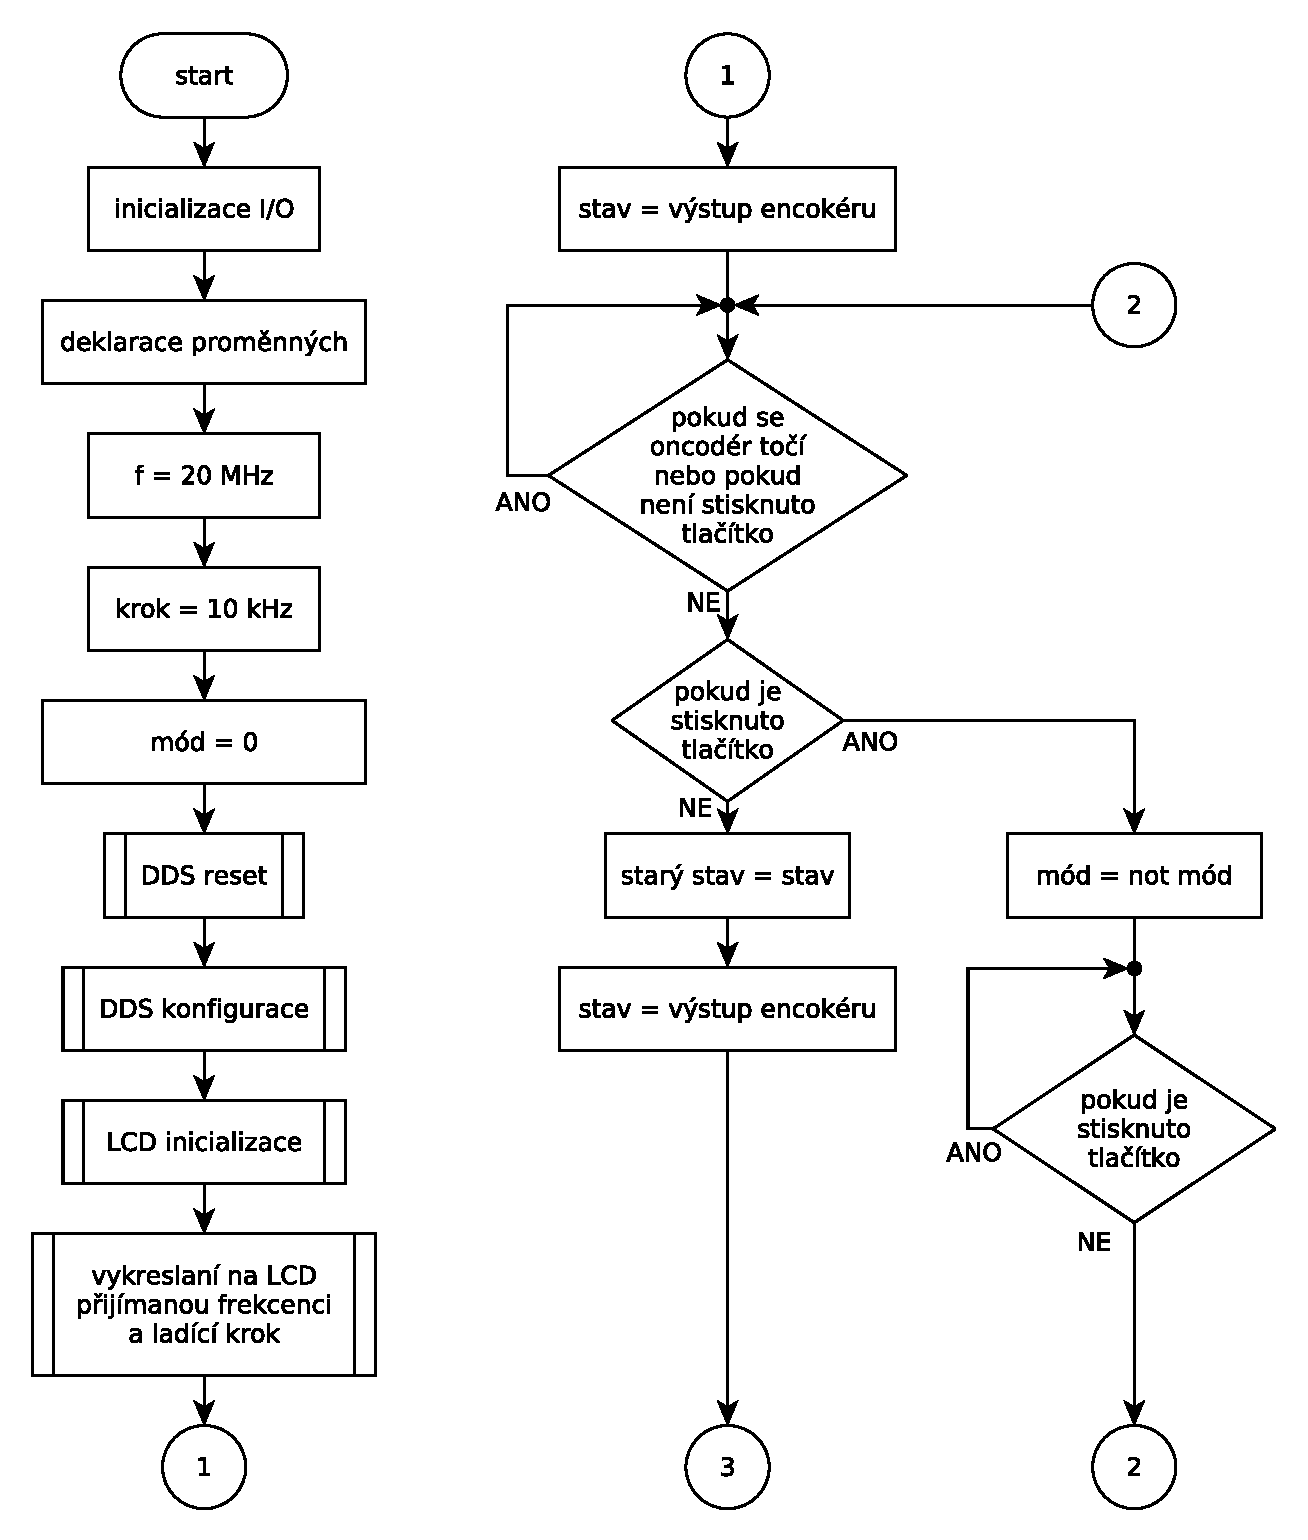
\includegraphics[height=150mm]{img/vyvojak_a.pdf}
	\caption{Vývojový diagram programu řídící jednotky část A}    		
\end{figure}

% vyvojak B
\begin{figure}[H]
	\centering
	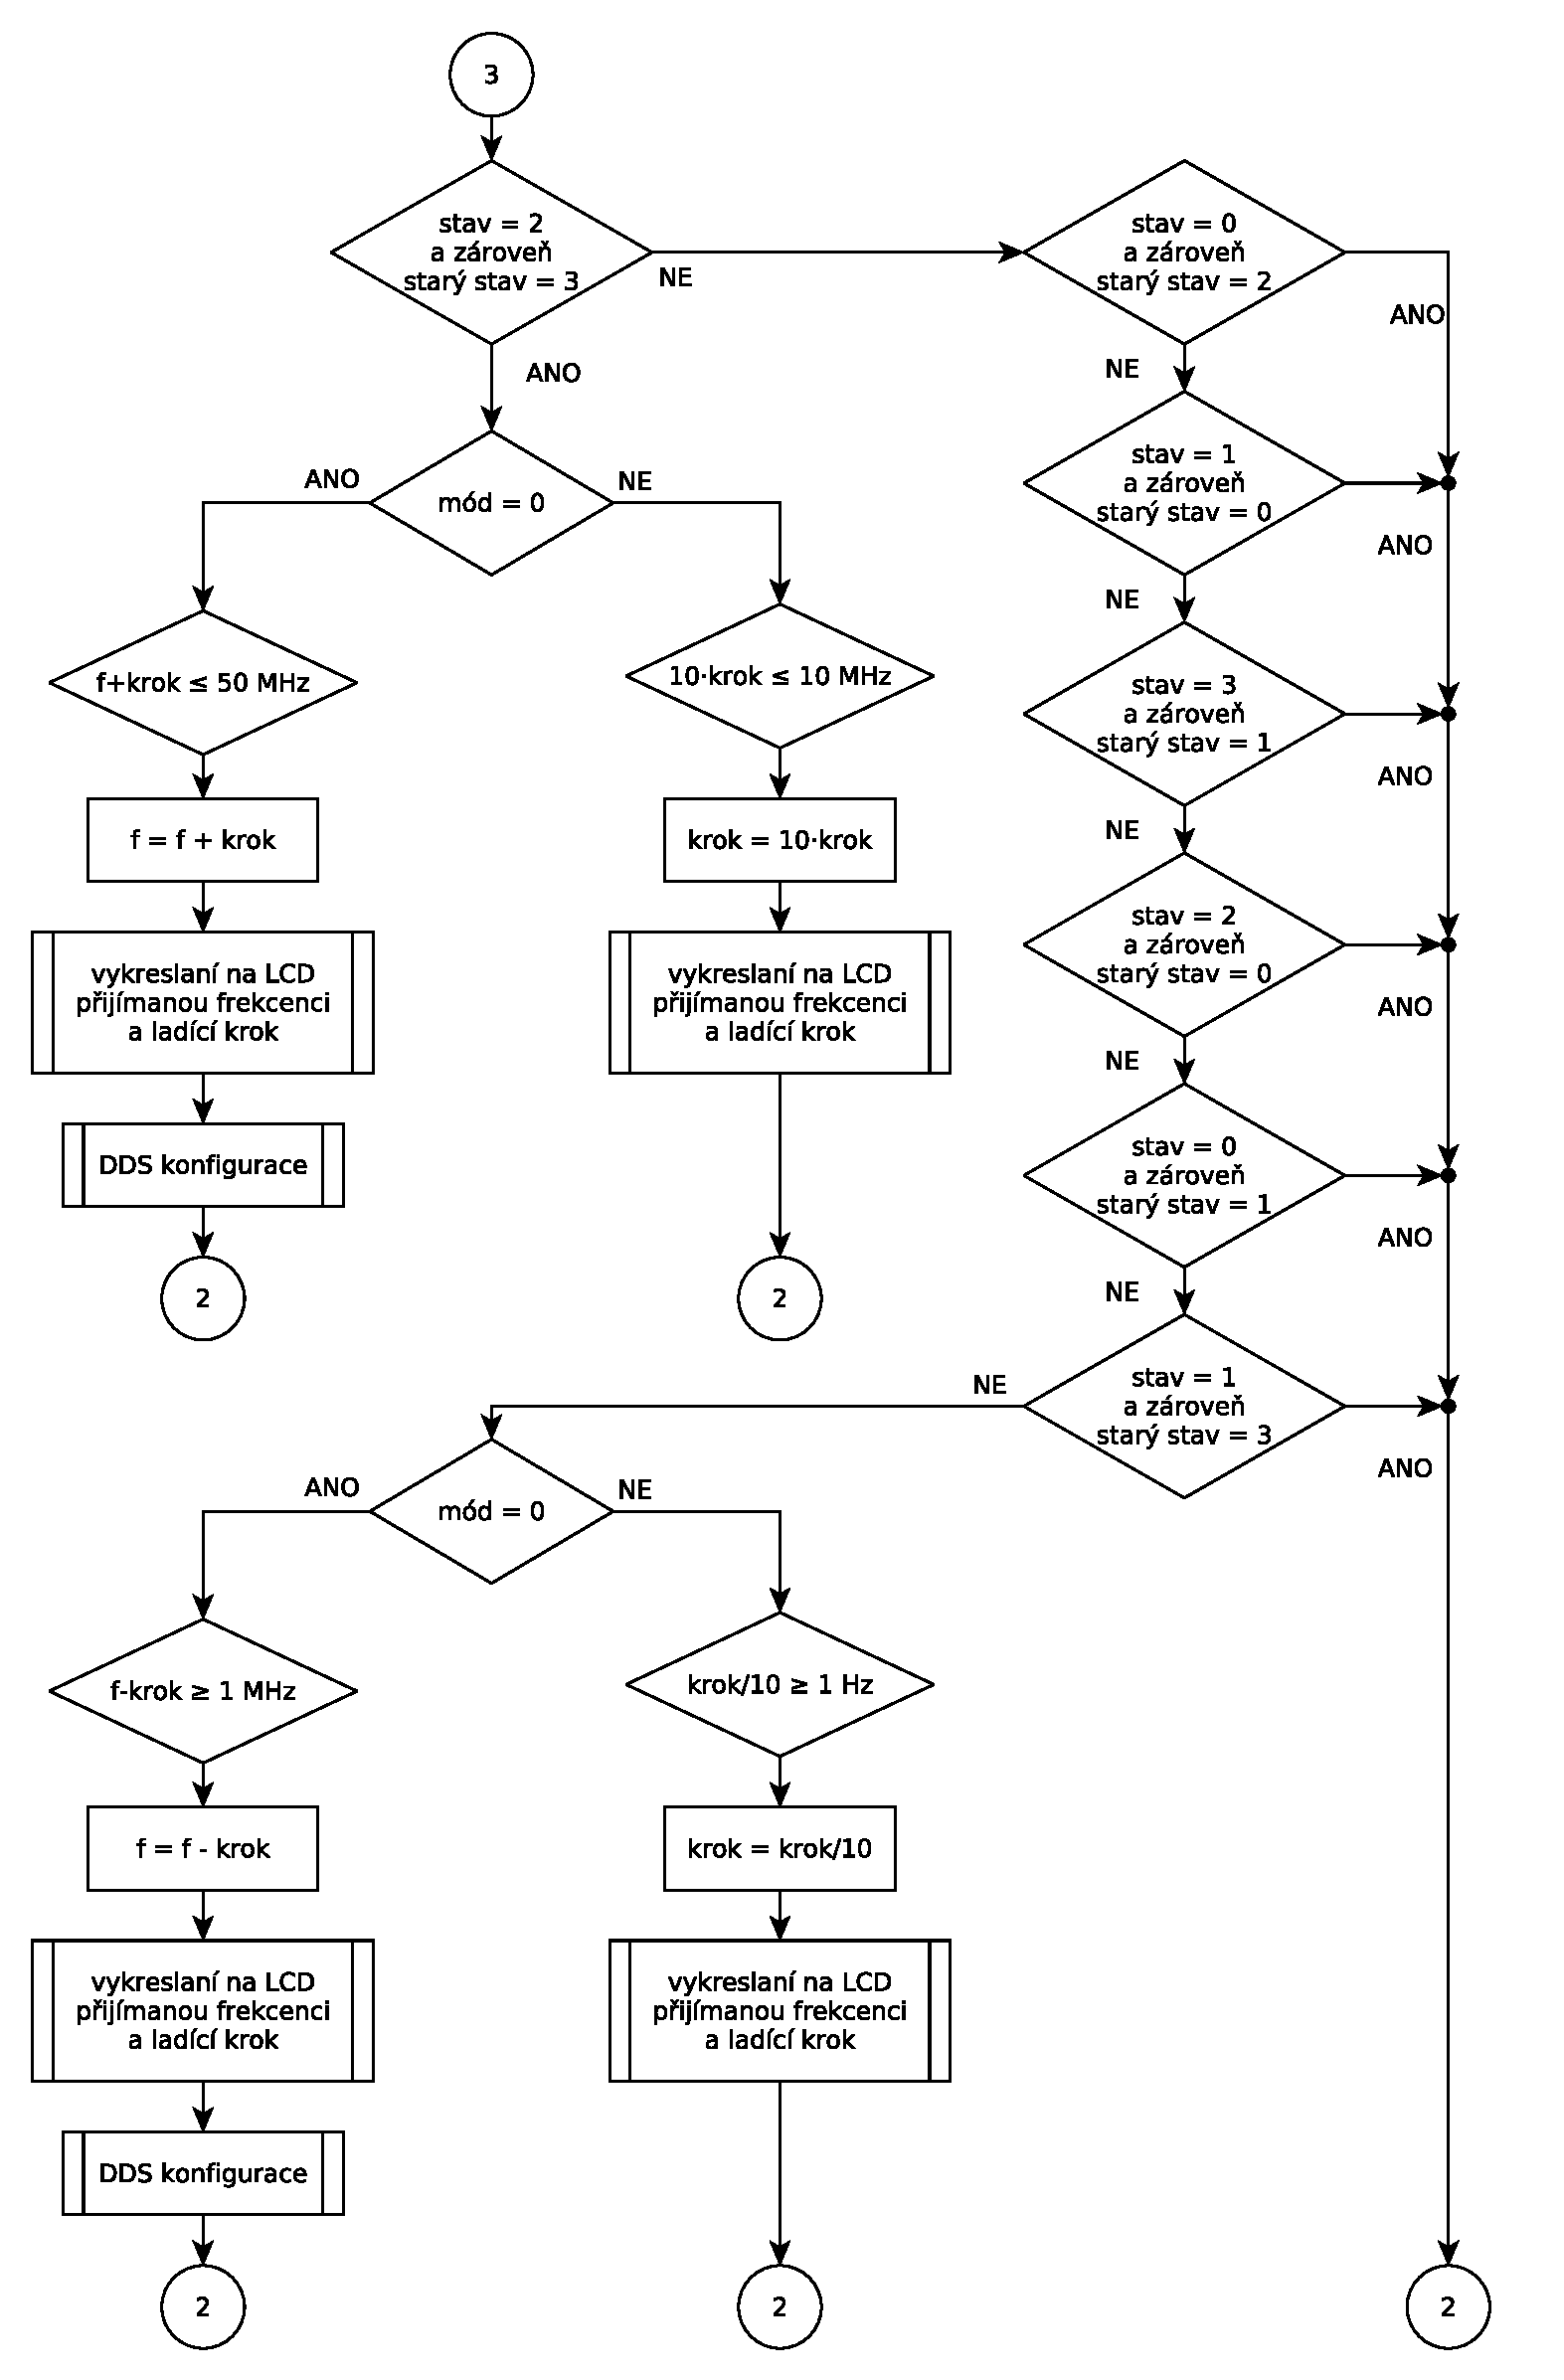
\includegraphics[height=220mm]{img/vyvojak_b.pdf}
	\caption{Vývojový diagram programu řídící jednotky část B}    		
\end{figure}


% schéma
\begin{landscape}
	\begin{figure}[h]
		\centering 	
		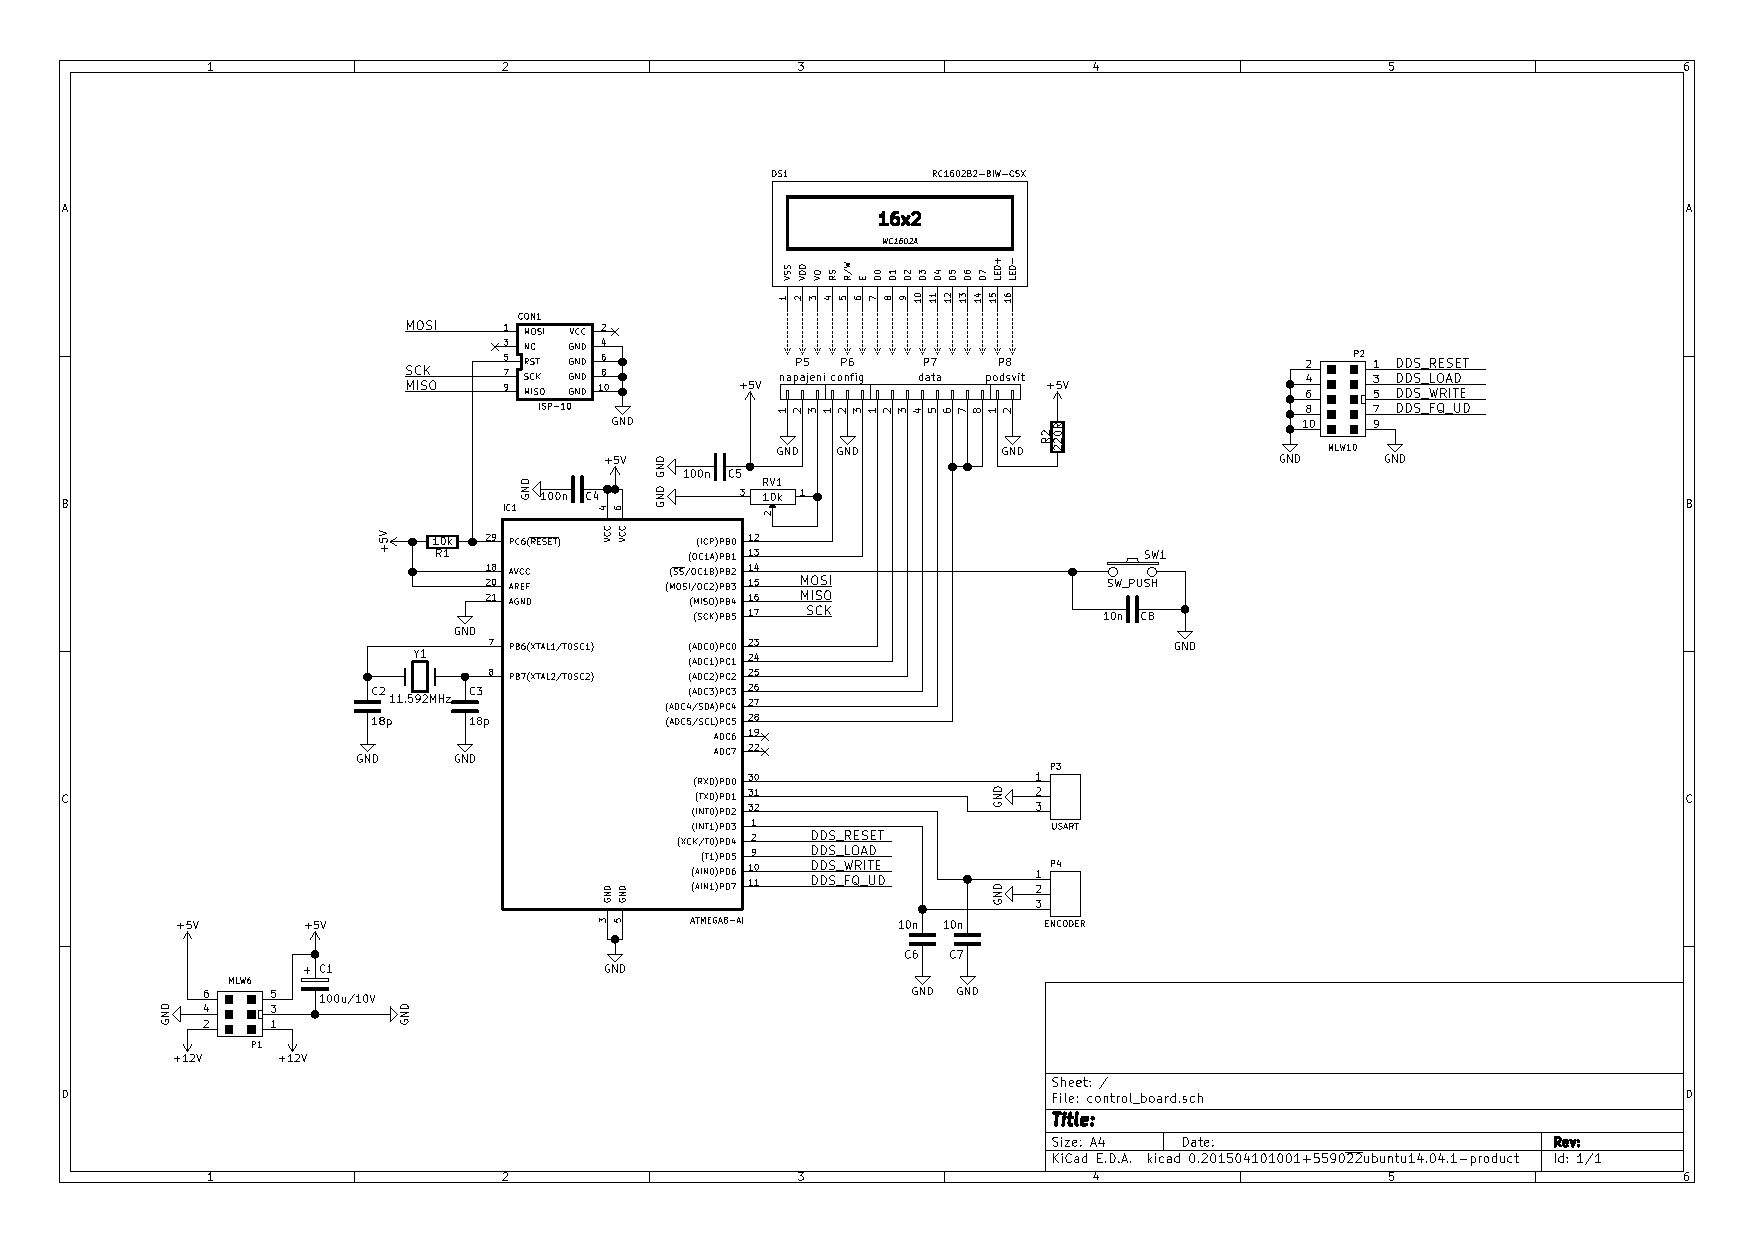
\includegraphics[height=\textwidth]{img/cu/sch.pdf}
		\caption{Schéma zapojení řídící jednotky}	
	\end{figure}
\end{landscape}
%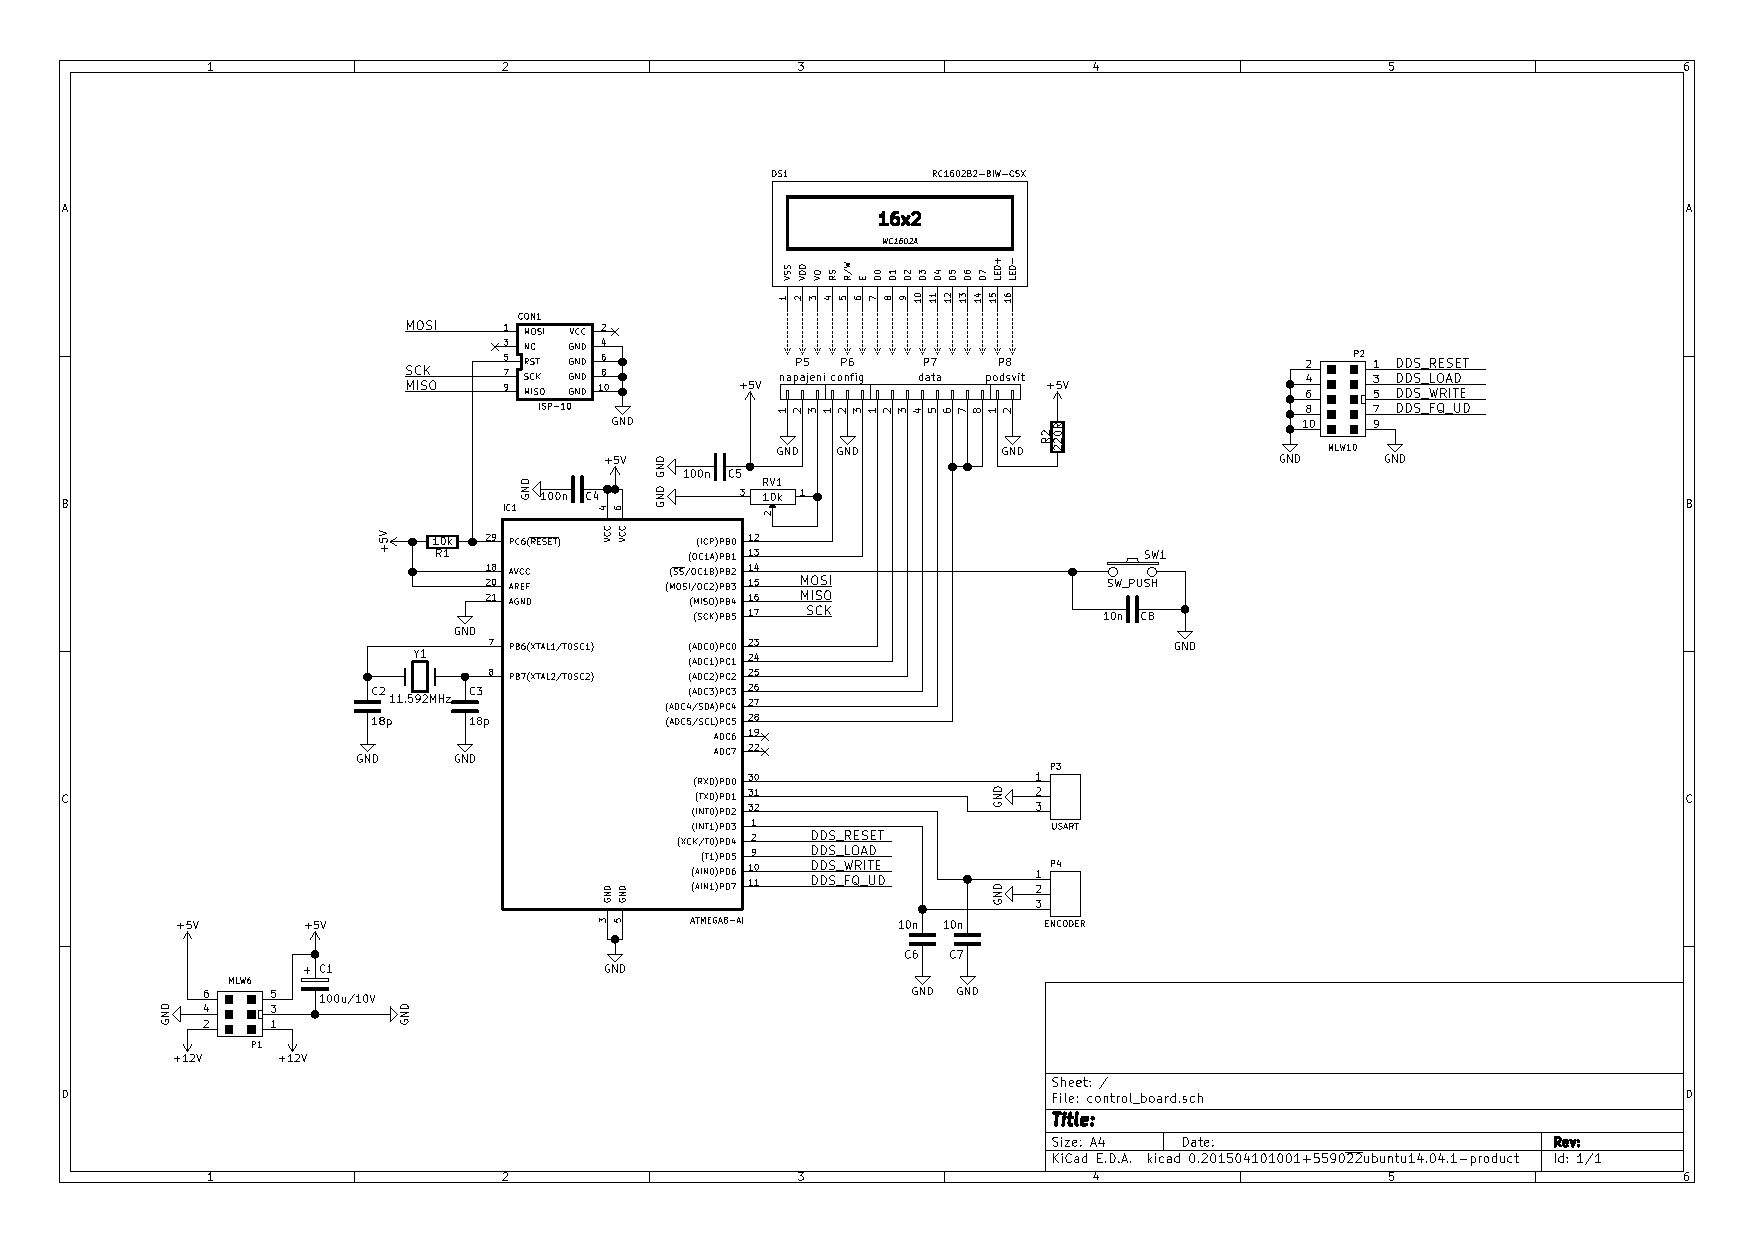
\includepdf[landscape=true]{img/cu/sch.pdf}

% DPS
\begin{figure}[H]
	\centering
	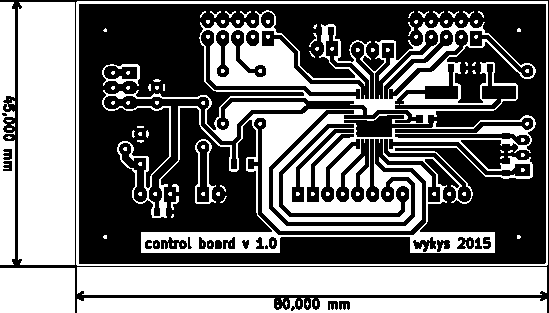
\includegraphics[width=170mm]{img/cu/cu_b.pdf}
	\caption{Deska plošného spoje řídící jednotky, strana spojů}    		
\end{figure}

% os f
\begin{figure}[H]
	\centering
	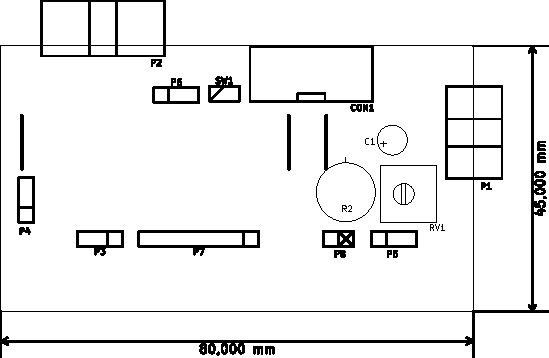
\includegraphics[width=170mm]{img/cu/os_f.pdf}
	\caption{Osazovací plán řídící jednotky, strana součástek}    		
\end{figure}

% os b
\begin{figure}[H]
	\centering
	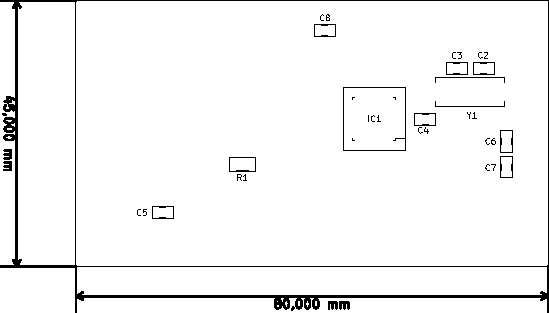
\includegraphics[width=165mm]{img/cu/os_b.pdf}
	\caption{Osazovací plán řídící jednotky, strana spojů}    		
\end{figure}

\begin{table}[H]
	\begin{center}
		\caption{Tabulka použitých součástek pro desku řídící jednotky}
		\label{tab:cu_os}      
		\begin{tabular}[H]{!{\vrule width 1pt}c|c|c|c!{\vrule width 1pt}}
		    \specialrule{1pt}{0pt}{0pt} 
		    \textbf{Určovatel}	&	\textbf{Pouzdro}	&	\textbf{Množství}	&	\textbf{Určení}	\\\specialrule{1pt}{0pt}{0pt} 
			C1	&	Elko\_vert\_11x5mm\_RM2.5\_CopperClear	&	1	&	100u/10V	\\\hline
			C2,C3	&	C\_0805	&	2	&	18p	\\\hline
			C4,C5	&	C\_0805	&	2	&	100n	\\\hline
			C6,C7,C8	&	C\_0805	&	3	&	10n	\\\hline
			CON1	&	vasch\_strip\_5x2	&	1	&	ISP-10	\\\hline
			IC1	&	TQFP-32\_7x7mm\_Pitch0.8mm	&	1	&	ATMEGA8-AI	\\\hline
			P1	&	vasch\_strip\_3x2\_90	&	1	&	MLW6	\\\hline
			P2	&	vasch\_strip\_5x2\_90	&	1	&	MLW10	\\\hline
			R1	&	R\_1206	&	1	&	10k	\\\hline
			RV1	&	Potentiometer\_Trimmer-Suntan-TSR-3386P	&	1	&	10k	\\\hline
			Y1	&	Crystal\_HC49-SD\_SMD	&	1	&	11.592MHz	\\\hline
			P5	&	pin\_socket\_3	&	1	&	napajeni	\\\hline
			P6	&	pin\_socket\_3	&	1	&	config	\\\hline
			P7	&	pin\_socket\_8	&	1	&	data	\\\hline
			P8	&	pin\_socket\_2	&	1	&	podsvit	\\\hline
			P4	&	pin\_strip\_3	&	1	&	ENCODER	\\\hline
			P3	&	pin\_strip\_3	&	1	&	USART	\\\hline
			SW1	&	pin\_strip\_2	&	1	&	SW\_PUSH	\\\hline
			R2	&	Resistor\_Vertical\_RM7.5mm	&	1	&	220R	\\\hline
			M1,M2,M3,M4	&	M3	&	4	&	M3	\\\specialrule{1pt}{0pt}{0pt} 
		\end{tabular}
	\end{center}
\end{table}

	
	\clearpage
\section{Lokální oscilátor}
%\subsection{Princip DDS}
\indent\indent Lokální oscilátor je postaven na obvodu od firmy Analog Devices AD9850BRS. Jedná se o takzvaný DDS - Direct Digital Synthesizer (přímá digitální syntéza) což je technologie určená pro generování, většinou harmonických signálů s digitálně přesně nastavitelným výstupním kmitočtem. Obvod AD9850 dokáže generovat, za předpokladu referenčního hodinového signálu o frekvenci $125~MHz$, sinusové průběhy od $0,0291~Hz$ s krokem $0,0291~Hz$. Integrovaný obvod se skládá z: rozhraní pro konfiguraci, registru pro zachycení vstupních dat, registru pro aktuální konfiguraci, DDS bloku, DAC a nízkošumového komparátoru.

Jak vlastně DDS funguje? DDS je tvořena pamětí nejčastěji ROM (Read Only Memory) ve které jsou uchovány vzorky funkce, kterou chceme generovat. V případě AD9850 jsou vzorky v rozlišení 10 bitů. Hodnota ve fázovém registru určuje o kolik vzorků se při dalším taktu referenčních hodin přesune. Když vnitřní čítač dosáhne konce paměti, dojde k jeho vynulování a pokračuje opět od začátku. Data z paměti jsou přiváděna  do rychlého 10 bitového DA převodníku, kde se převádí na napětí.  			
  			
DDS Obvod se podle obdrženého konfiguračního slova nastaví do odpovídajícího módu a pokud jsou konfigurační data v pořádku, je na výstupu DA převodníku požadovaný signál odpovídající nastavenému kmitočtu.

% blokáč AD9850
\begin{figure}[H]
	\centering
	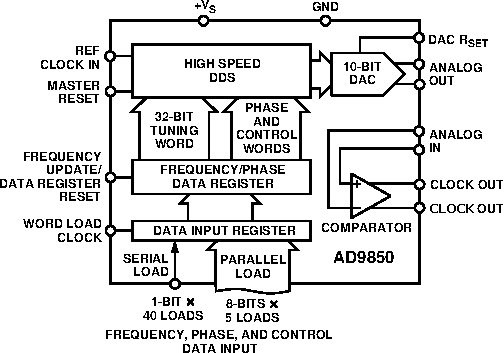
\includegraphics[width=140mm]{img/lo/AD9850_bd.pdf}
	\caption{Blokové schéma AD9850}    		
\end{figure}

\clearpage

\subsection{Výpočet konfiguračního slova}
\indent\indent Konfigurační slovo má 40 bitů a slouží k nastavení výstupní frekvence a módu práce DDS. První 4 byte určují požadovaný kmitočet a poslední byte určuje mód. Hodnota 32b slova pro konfiguraci frekvence se vypočítá podle vztahu:
  			$$f_{OUT} = \frac{\Delta Phase \cdot CLKIN}{2^{32}}$$
  			
  			\hspace*{2cm}kde:\newline    
  			\hspace*{4cm}$f_{OUT}$ \dotfill požadovaná výstupní frekvence\hspace*{4cm}\newline
		  	\hspace*{4cm}$\Delta Phase$ \dotfill 32b konfigurační slovo\hspace*{4cm}\newline
		  	\hspace*{4cm}$CLKIN$ \dotfill frekvence referenčních hodin\hspace*{4cm}\newline
		  	
		  	
		  	Poslední byte konfiguračního slova přepíná DDS do čtyřech módů práce:
		  	
		  	\begin{table}[H]
    			\begin{center}
    				\caption{Možné módy obvodu AD9850}
      				\label{tab:lo_mod}      
					\begin{tabular}[H]{!{\vrule width 1pt}c|c!{\vrule width 1pt}}
				        \specialrule{1pt}{0pt}{0pt} 
				        \textbf{Hodnota} & \textbf{Popis} \\\specialrule{1pt}{0pt}{0pt} 
				        $4$ &	power-down	\\\hline 				
				        $0$ &	power-up	\\\hline 
				        $2$ &	test		\\\hline 
				        $1$ &	test
						\\\specialrule{1pt}{0pt}{0pt}         
		    		\end{tabular}     				
    			\end{center}
  			\end{table}
  			
  			Když je tato posloupnost vytvořena, tak je buď pomocí sériového nebo paralelního rozhraní nahrána do DDS.

\subsubsection{Konfigurace DDS}
\indent\indent Aby AD9850 správně fungoval, je třeba jej napřed správně nakonfigurovat. K tomuto účelu je možné přistupovat dvěma způsoby. První způsob je pomocí paralelního rozhraní a druhý pomocí rozhraní sériového.
  		
\subsubsection{Konfigurace pomocí paralelního rozhraní}
\indent\indent Ke konfiguraci se používá 8 bitového datová sběrnice pro přenos dat, k ovládání komunikace slouží řídící signály: WRITE, FQ\_UD a RESET. Komunikace probíhá po jednotlivých bytech. Napřed je třeba obvod resetovat. To se provede přivedením logické úrovně H na signál RESET po dobu minimálně pěti period referenčních hodin. Tím se vynuluje ukazatel registru zachycení a DDS je připravena k zápisu konfiguračního slova. Konfigurační slovo o délce 40b neboli 5B je posloupnost určující výstupní frekvenci,  fázi a mód. Zápis probíhá tak, že na datovou sběrnici nastavíme byte (začíná se od LSB směrem k MSB). Poté vyšleme zapisovací impuls na signál WRITE široký minimálně $3,5~ns$. Data jsou zapsána do záchytného registru pro konfiguraci při náběžné hraně. Poté počkáme minimálně $3,5~ns$ (během tohoto času se zvyšuje ukazatel do záchytné paměti vstupních dat) a můžeme pokračovat. Tento proces je nutné zopakovat celkem pětkrát aby se celé konfigurační slovo přeneslo do DDS. Nakonec se celé konfigurační slovo uloží do řídícího registru DDS. Toto se provede přivedením impulzu na vstup FQ\_UD.
  			
\subsubsection{Konfigurace pomocí sériového rozhraní}
\indent\indent Sériová konfigurace na rozdíl od paralelní využívá pro přenos dat jen jeden datový signál a to sedmý bit D7 komunikační sběrnice označovaný jako LOAD a dále používá signály CLK, FQ\_UD a RESET. Aby bylo možné komunikovat po sériové sběrnici je nutné připojit datové signály komunikační sběrnice D0 a D1 na logickou úroveň H a signál D2 na logickou úroveň L. Sériová komunikace tedy probíhá po jednotlivých bitech. Na začátku je opět nutné AD9850 restartovat, přivedením logické úrovně H na signál RESET po dobu alespoň pěti period hodinového signálu. Dále je třeba inicializovat sériovou komunikaci. Inicializace probíhá přivedením pulsu na signál CLK o minimální šířce $3,5~ns$ počkáním alespoň $3,5~ns$ a přivedením pulsu minimální šířky $7~ns$ na FQ\_UD. Po této inicializaci následuje přenos konfiguračního slova. Zápis konfiguračního slova probíhá následovně. Na signál LOAD nastavujeme jednotlivé konfigurační bity (od LSb do MSb). Když je na signálu LOAD stabilní hodnota aktuálně přenášeného bitu, tak vyšleme puls na CLK široký alespoň $3,5~ns$. Při náběžné hraně se zapíše bit do registru pro zachycení konfiguračního slova. Poté čekáme minimálně $3,5~ns$, během tohoto intervalu se inkrementuje ukazatel do registru pro zachycení konfiguračního slova o jedničku. Tento postup opakujeme celkem čtyřicet krát. V záchytném registru je zapsáno celé konfigurační slovo. Nyní se přivedením zapisovacího impulzu o minimální šířce $7~ns$ na vstup FQ\_UD, provede zápis do řídícího registru DDS.
  			
\subsection{Popis funkce bloku}
\indent\indent Jak již bylo zmíněno výše, pro správnou funkci generátoru DDS, je potřeba použít stabilní zdroj hodinového signálu. Z tohoto důvodu je použit stabilní krystalový oscilátor CFPS-73-100M který dodává kmitočet $100~MHz$. Signál generovaný krystalovým oscilátorem je však sinusového průběhu a pro potřeby zdroje hodinového signálu pro DDS je ho potřeba upravit. Tato úprava spočívá v předřazeném tvarovači, který je tvořen rychlým hradlem NAND se Schmittovým vstupním obvodem a je zapojeno jako invertor. Jako vhodný typ hradla se ukázal obvod 74VHC1G132DTTG, což je jedno hradlo NAND se Schmittovým vstupem v pouzdře SOT 23-5. 
Pro zabezpečení ochrany obvodu DDS, je na vstup datových signálů předřazen rychlý oddělovač sběrnice 74F245. Analogový vystup je přiveden k dolní propusti tvořenou L1, C8 a C9. Tento filtr slouží k potlačení vyšších harmonických kmitočtů, které vznikají jako vedlejší produkt digitální syntézy. Současně také upravuje impedanci pro koncový zesilovací stupeň realizovaný s tranzistorem KF630D. Jeho obvodové řešení je shodné se zesilovacím stupněm ve vstupním předzesilovacím selektivním zesilovači. Transformátor TR1 je proveden na toroidním jádře z hmoty N2, jako bifilární vinutí se sedmi závity.

% schéma
\begin{landscape}
	\begin{figure}[h]
		\centering 	
		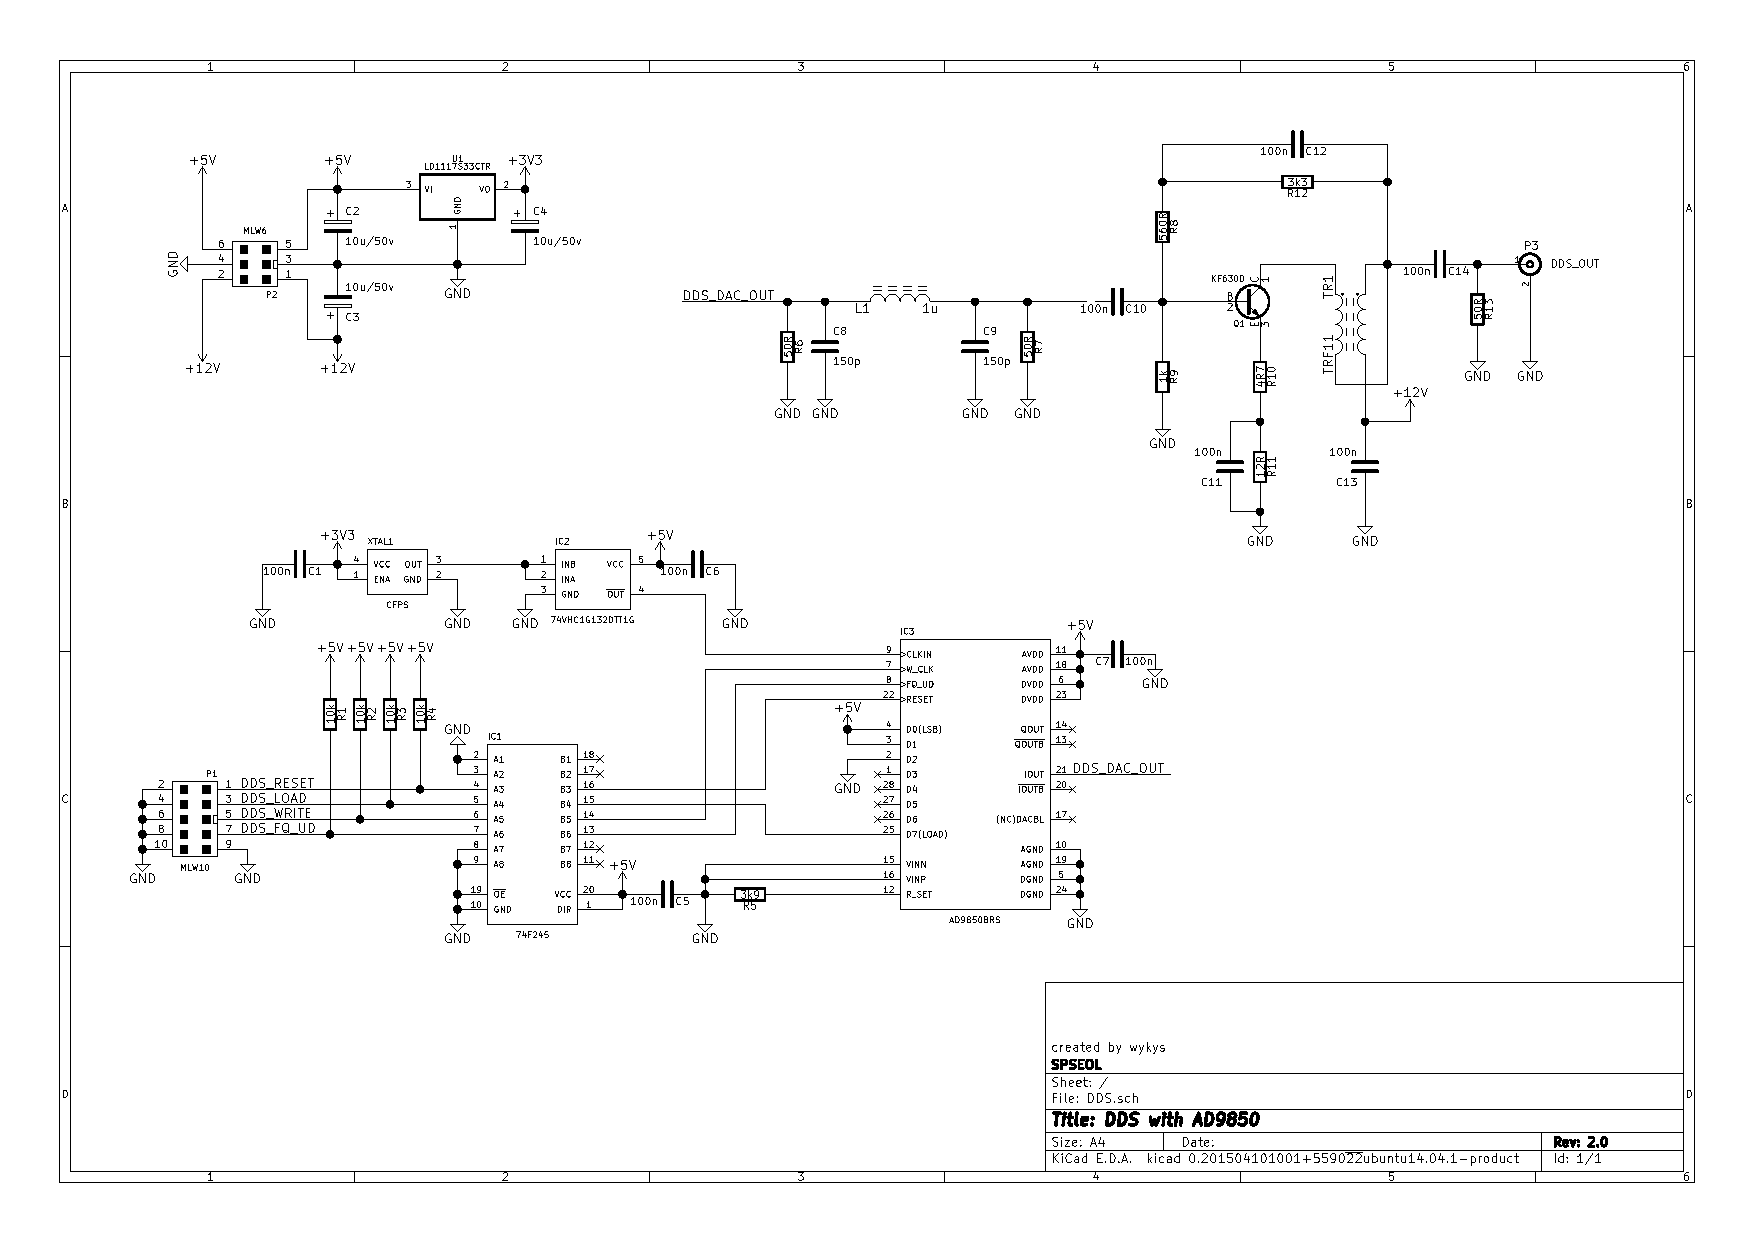
\includegraphics[height=\textwidth]{img/lo/sch.pdf}
		\caption{Schéma zapojení řídící jednotky}	
	\end{figure}
\end{landscape}
%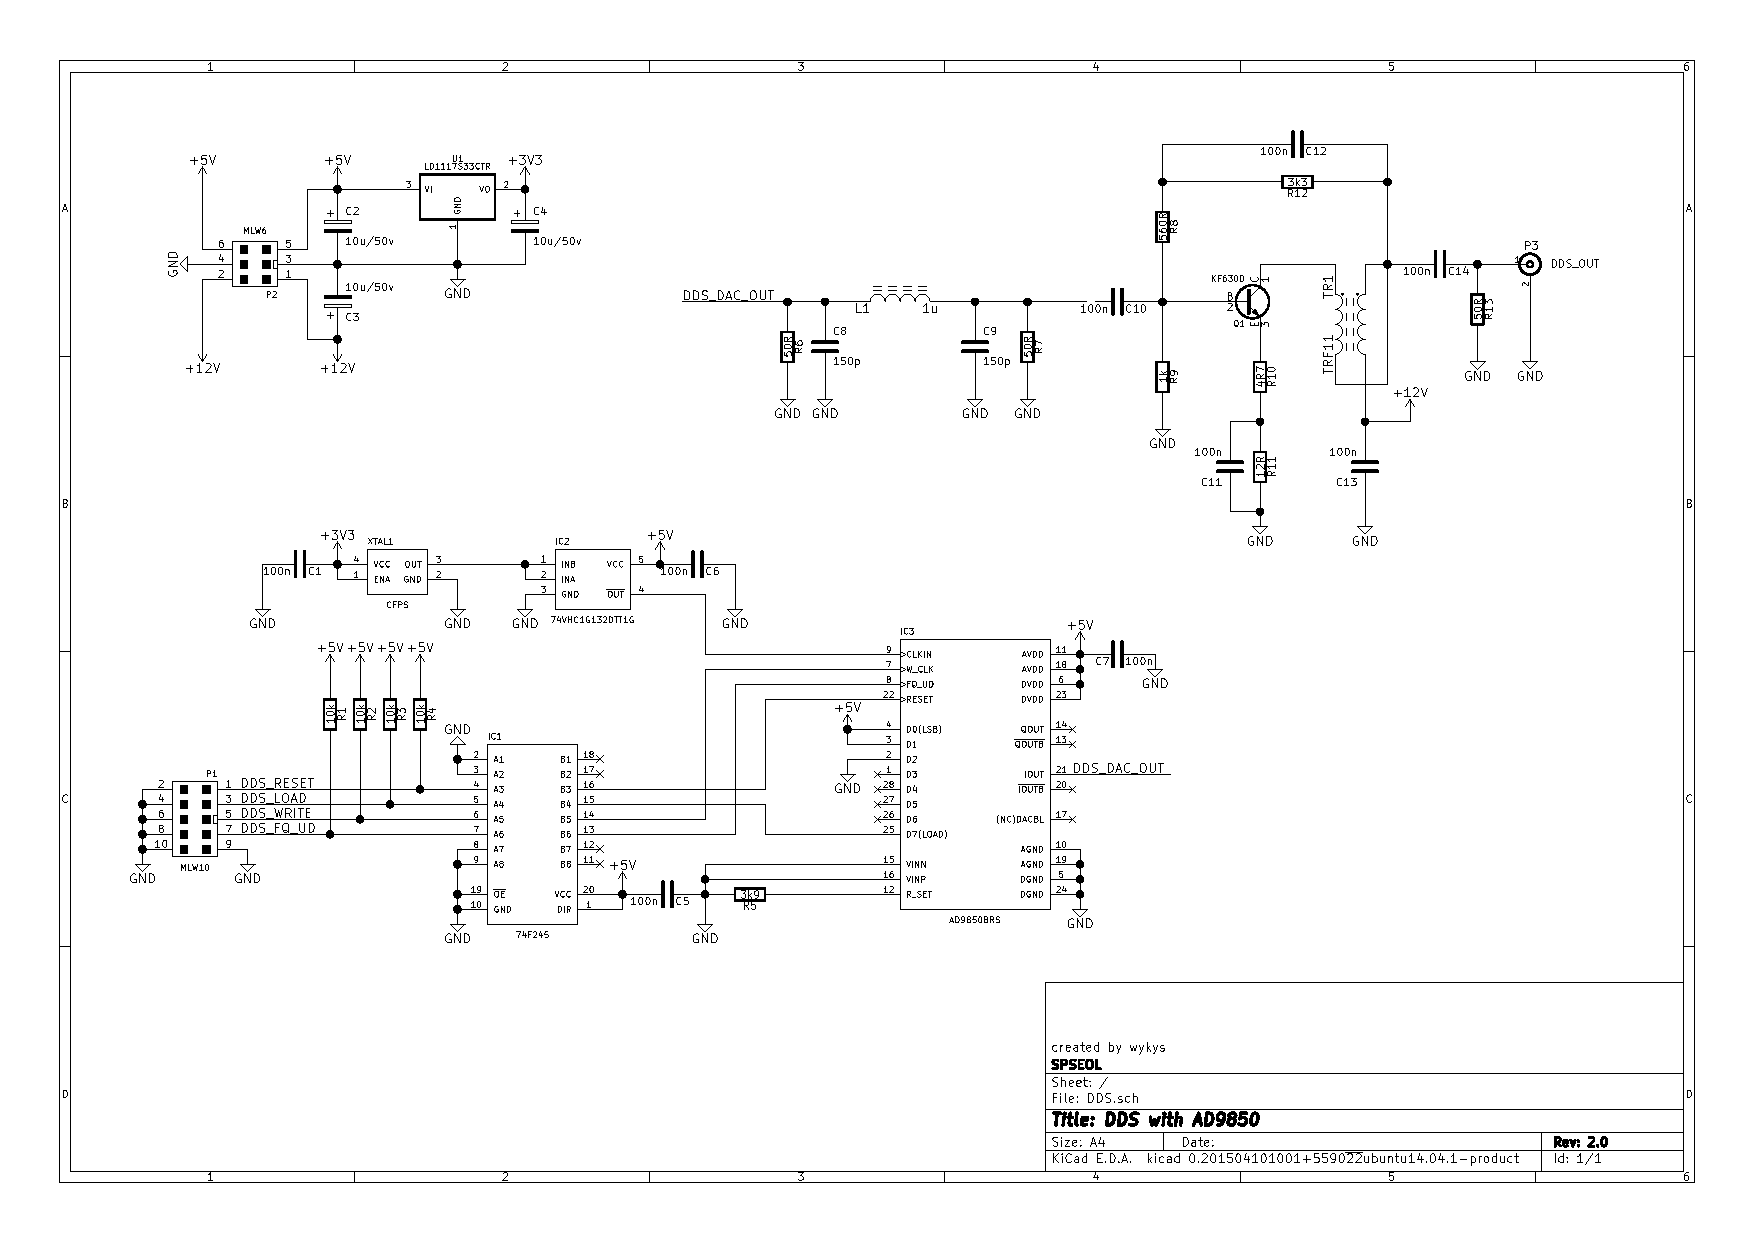
\includepdf[landscape=true]{img/lo/sch.pdf}

% DPS
\begin{figure}[H]
	\centering
	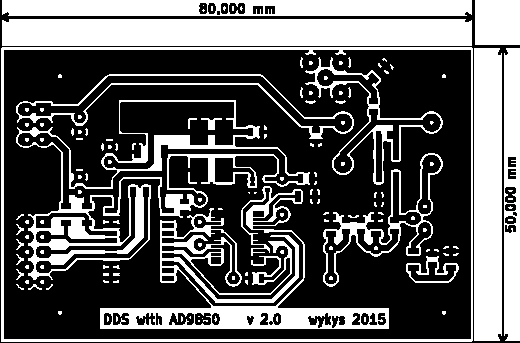
\includegraphics[width=160mm]{img/lo/cu_b.pdf}
	\caption{Deska plošného spoje lokálního oscilátoru, strana spojů}    		
\end{figure}

% os f
\begin{figure}[H]
	\centering
	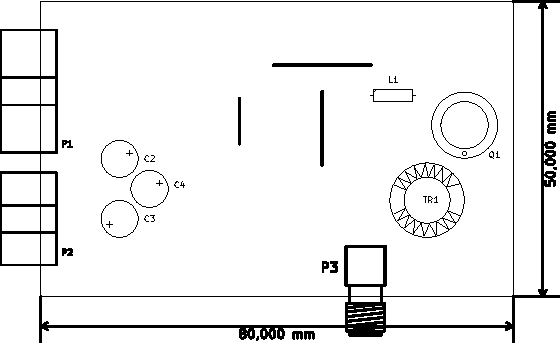
\includegraphics[width=160mm]{img/lo/os_f.pdf}
	\caption{Osazovací plán lokálního oscilátoru, strana součástek}    		
\end{figure}

% os b
\begin{figure}[H]
	\centering
	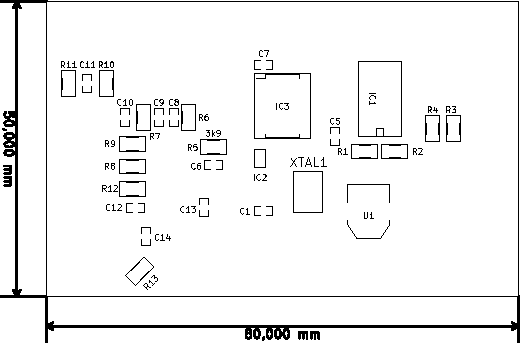
\includegraphics[width=120mm]{img/lo/os_b.pdf}
	\caption{Osazovací plán lokálního oscilátoru, strana spojů}    		
\end{figure}

\begin{table}[H]
	\begin{center}
		\caption{Tabulka použitých součástek pro desku lokálního oscilátoru}
		\label{tab:lo_os}     
		\begin{tabular}[H]{!{\vrule width 1pt}c|c|c|c!{\vrule width 1pt}}
		    \specialrule{1pt}{0pt}{0pt} 
		    \textbf{Určovatel}	&	\textbf{Pouzdro}	&	\textbf{Množství}	&	\textbf{Určení}	\\\specialrule{1pt}{0pt}{0pt} 			
			C1,C5-C7,C10-C14	&	SMD-0805	&	9	&	100n	\\\hline
			C2,C3,C4	&	Elko\_vert\_11.2x6.3mm\_RM2.5	&	3	&	10u/50v	\\\hline
			C8,C9	&	SMD-0805	&	2	&	150p	\\\hline
			IC1	&	SO-20-L	&	1	&	74F245	\\\hline
			IC2	&	SOT-23-5	&	1	&	74VHC1G132DTT1G	\\\hline
			L1	&	R3-LARGE\_PADS	&	1	&	1u	\\\hline
			Q1	&	TO5	&	1	&	KF630D	\\\hline
			R1,R2,R3,R4	&	R\_1206	&	4	&	10k	\\\hline
			R5	&	R\_1206	&	1	&	3k9	\\\hline
			R6,R7,R13	&	R\_1206	&	3	&	50R	\\\hline
			R8	&	R\_1206	&	1	&	560R	\\\hline
			R9	&	R\_1206	&	1	&	1k	\\\hline
			R10	&	R\_1206	&	1	&	4R7	\\\hline
			R11	&	R\_1206	&	1	&	12R	\\\hline
			R12	&	R\_1206	&	1	&	3k3	\\\hline
			TR1	&	Amidon-T44-2	&	1	&	TRF11	\\\hline
			U1	&	SOT-223	&	1	&	LD1117S33CTR	\\\hline
			P3	&	MCX	&	1	&	DDS\_OUT	\\\hline
			P1	&	vasch\_strip\_5x2\_90	&	1	&	MLW10	\\\hline
			P2	&	vasch\_strip\_3x2\_90	&	1	&	MLW6	\\\hline
			M1,M2,M3,M4	&	M3	&	4	&	M3	\\\hline
			IC3	&	SSOP-28	&	1	&	AD9850BRS	\\\hline
			XTAL1	&	SMD7x5	&	1	&	CFPS	\\\specialrule{1pt}{0pt}{0pt} 
		\end{tabular}	 
	\end{center}
\end{table}


	\clearpage
\section{Směšovací blok}
\indent\indent Tento obvod má za úkol frekvenčně posunout přijímaný napěťový signál do základního nízkofrekvenčního (audio) pásma, tak aby jej bylo možné zpracovávat pomocí zvukové karty. Výstupem s tohoto modulu jsou dva signály I a Q navzájem posunuty o $\frac{\pi}{2}$. Signály I a Q jsou přiváděny na linkový vstup zvukové karty.

\subsection{Popis funkce bloku}
\indent\indent Do obvodu vstupují dva napěťové signály, jeden s lokálního oscilátoru a druhý ze selektivního zesilovače. Signál ze selektivního zesilovače jde přes rekonstrukční filtr s mezní frekvencí $35~MHz$, který odstraňuje vysokofrekvenční šum a vyšší harmonické frekvence, které nepotlačil první rekonstrukční filtr po digitální syntéze.

% rekonstrukční filtr
\begin{figure}[H]
	\centering
	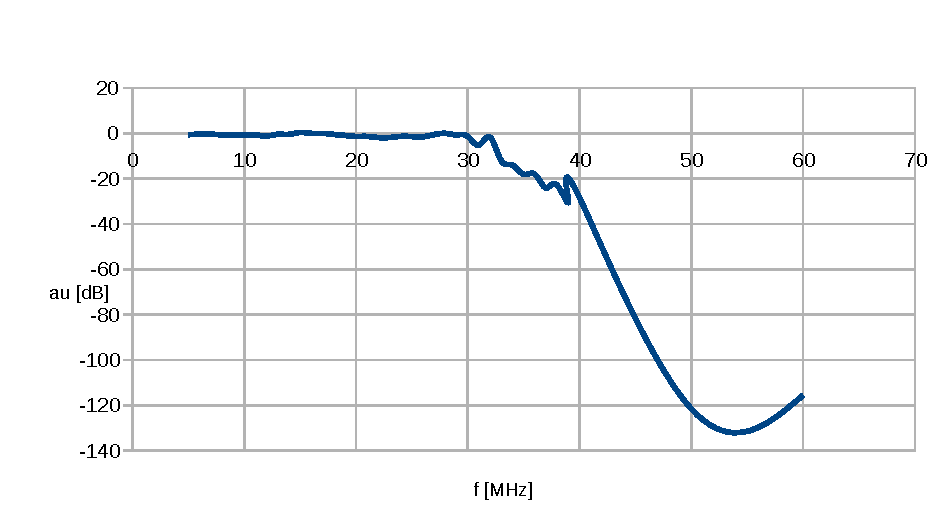
\includegraphics[width=170mm]{img/mix/filtr.pdf}
	\caption{Graf napěťového přenosu rekonstrukčního filtru}    		
\end{figure}

Signál je přiveden do diodového kruhového směšovače, ten ale potřebuje, aby vstupní signál měl úroveň nejméně $7~dBm$. Proto je zesílen v třístupňovém zesilovači, tvořeném kaskádově řazenými zesilovači, pracujícími ve třídě A. Nejprve se signál zesiluje napěťově v prvních dvou stupních postavených s tranzistory KF190, poté je signál výkonově zesílen v zesilovači založeném opět na tranzistoru KF630D. Tento zesilovač je opět obdobný, jako vstupní zesilovač popsaný ve druhé kapitole, s tím rozdílem, že transformátor je tentokrát navinutý na toroidním jádru s materiálu N5. Po zesílení je signál přiveden do již zmíněného diodového kruhového směšovače, založeném na rychlých Schottkyho diodách KAS44 a transformátorech T4 a T5. KAS44 je diodový směšovač. Uvnitř KAS44 se nacházejí čtyři vyvážené diody. Po smíšení je signál přiveden na paralelní pásmovou propust, skládající se ze dvou rezonančních obvodů. První rezonanční obvod se skládá z kondenzátorů C17, C18 a T2 a je naladěn na $5,7~MHz$. Druhý rezonanční obvod se skládá z kondenzátorů C12, C13 a transformátoru T1. Tento obvod rezonuje na kmitočtu $6,0~MHz$. Paralelní obvody spojuje dohromady vazební kondenzátor C16. Za touto pásmovou frekvencí je tedy mezifrekvence k kmitočtu $5,7-6,0~MHz$. Tento mezifrekvenční signál je dále zpracováván. Křemíkový oscilátor XTAL1 rezonuje na frekvenci $24,0~MHz$ a vytváří sinusové napětí. Sinusové napětí s křemíkového oscilátoru je opět vytvarováno tvarovačem impulzů tvořeným integrovaným obvodem IC1. Poté upravený hodinový signál pokračuje do integrovaného obvodu U1. U1 je obvod 74F74, který má v sobě integrované dva klopné obvody typu D. U1 je zapojen jako 2b Johnsův čítač, to znamená, že na výstupu generuje dva signály navzájem posunuté o $\frac{\pi}{2}$. Během čtyř taktů oscilátoru se na výstupu Johnsova čítače prostřídají všechny možné stavy. Výstup Johnsova čítače je použit jako adresový vstup pro obvod U3. U3 je digitálně řízený přepínač založený na technologii MOS-FET. U3 postupně přepíná své 4 polohy. Na vstupu přepínače je přiveden mezifrekvenční signál. Na spínače obvodu U3 jsou připojeny kondenzátory C22, C25, C26 a C28. Slouží zde jako analogová paměť. Každý kondenzátor je jednou za periodu  mezifrekvence sepnut a nabíjen. Přepínání poloh spínačů a následné nabíjení kondenzátorů jsou posunuty v čase o $\frac{\pi}{2}$. Tím, že jsou kondenzátory spínány dochází ke směšování. Jedná se o podobnou myšlenku jako při spínání diody, s tím rozdílem, že kondenzátor  je nabíjen a pak se po zbytek času vybíjí. Na kondenzátorech jsou tedy čtyři napěťové průběhy posunuté o $\frac{\pi}{2}$ v nízko frekvenčním pásmu. Proto se tomuto zapojení říká kvadraturní detektor. (Podle svého objevitele někdy též nazývaný Tayloe detector). Vzhledem k tomu že na výstupu jsou signály posunuty o $\frac{\pi}{2}$, tak je zjevné, že dva z nich nesou redundantní informaci. Tedy na kondenzátoru C22 je napěťový průběh posunut o $\frac{\pi}{2}\pi$. Na kondenzátoru C25 je ten samý průběh ale posunutý o $\frac{3\pi}{2}$. Tedy v podstatě invertovaný průběh co je na kondenzátoru C22. Proto jsou tyto dvě napětí přivedeny do diferenciálního zesilovače postaveném na operačním zesilovači U4. U4 je špičkový operační zesilovač AD8055 s nízkým zkreslením a šumem, pracující až do frekvence $300~MHz$. Díky tomu, že jsme sečetli redundantní signál se signálem který jsme potřebovali, tak jsme dostali na výstupu zesílený signál. Obdobně se zpracují zbylé dva signály po kvadraturním směšování z kondenzátorů C26 a C28. Na těchto kondenzátorech jsou napěťové průběhy posunuty o $0\pi$ a $\pi$. Za diferenciálními zesilovači jdou tantalové kondenzátory C34 a C35, které slouží k oddělení stejnosměrné složky od střídavých napěťových signálů a snižují  offset při následné digitalizaci signálu ve zvukové kartě. Za kondenzátory C34 a C35 jsou tedy již signály I a Q, které slouží k softwarové demodulaci.

% schéma
\begin{landscape}
	\begin{figure}[h]
		\centering 	
		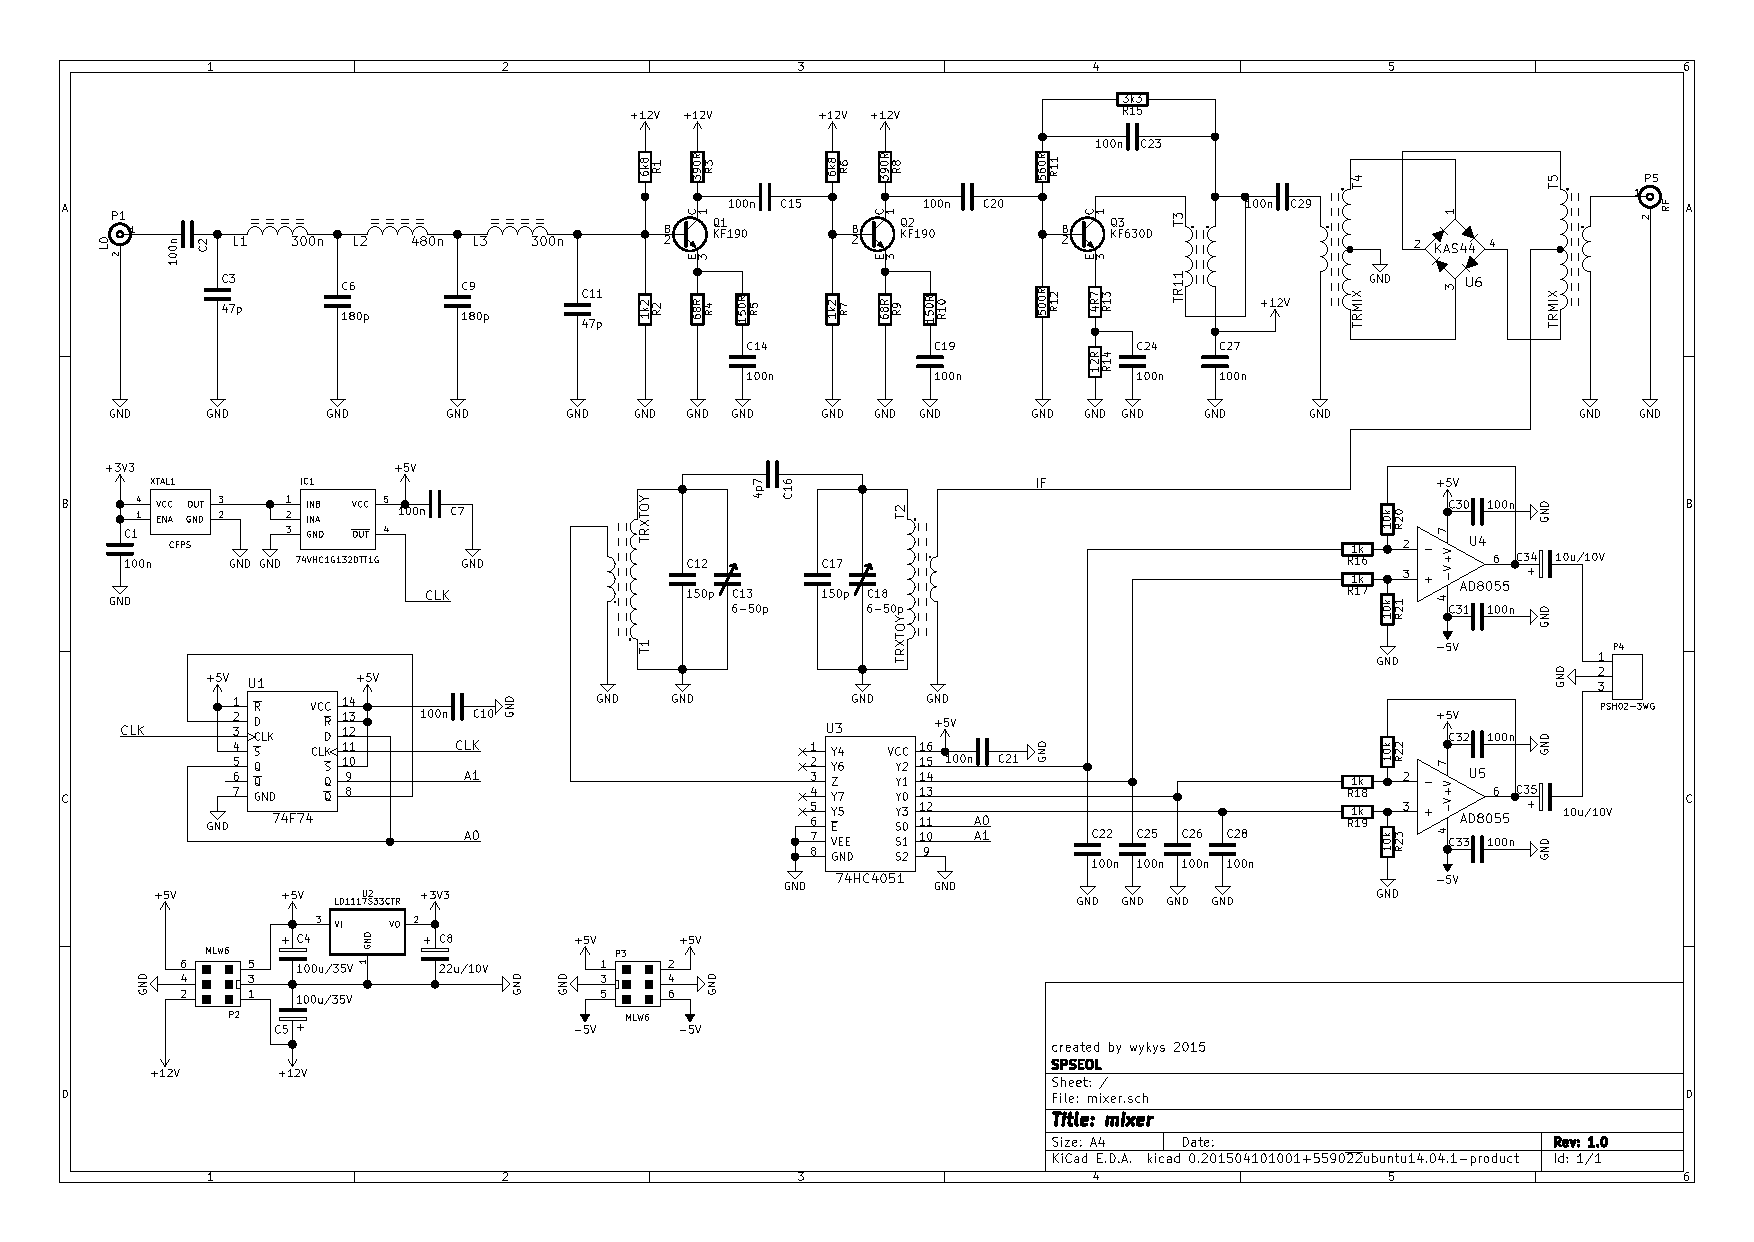
\includegraphics[height=\textwidth]{img/mix/sch.pdf}
		\caption{Schéma zapojení směšovacího bloku}	
	\end{figure}
\end{landscape}
%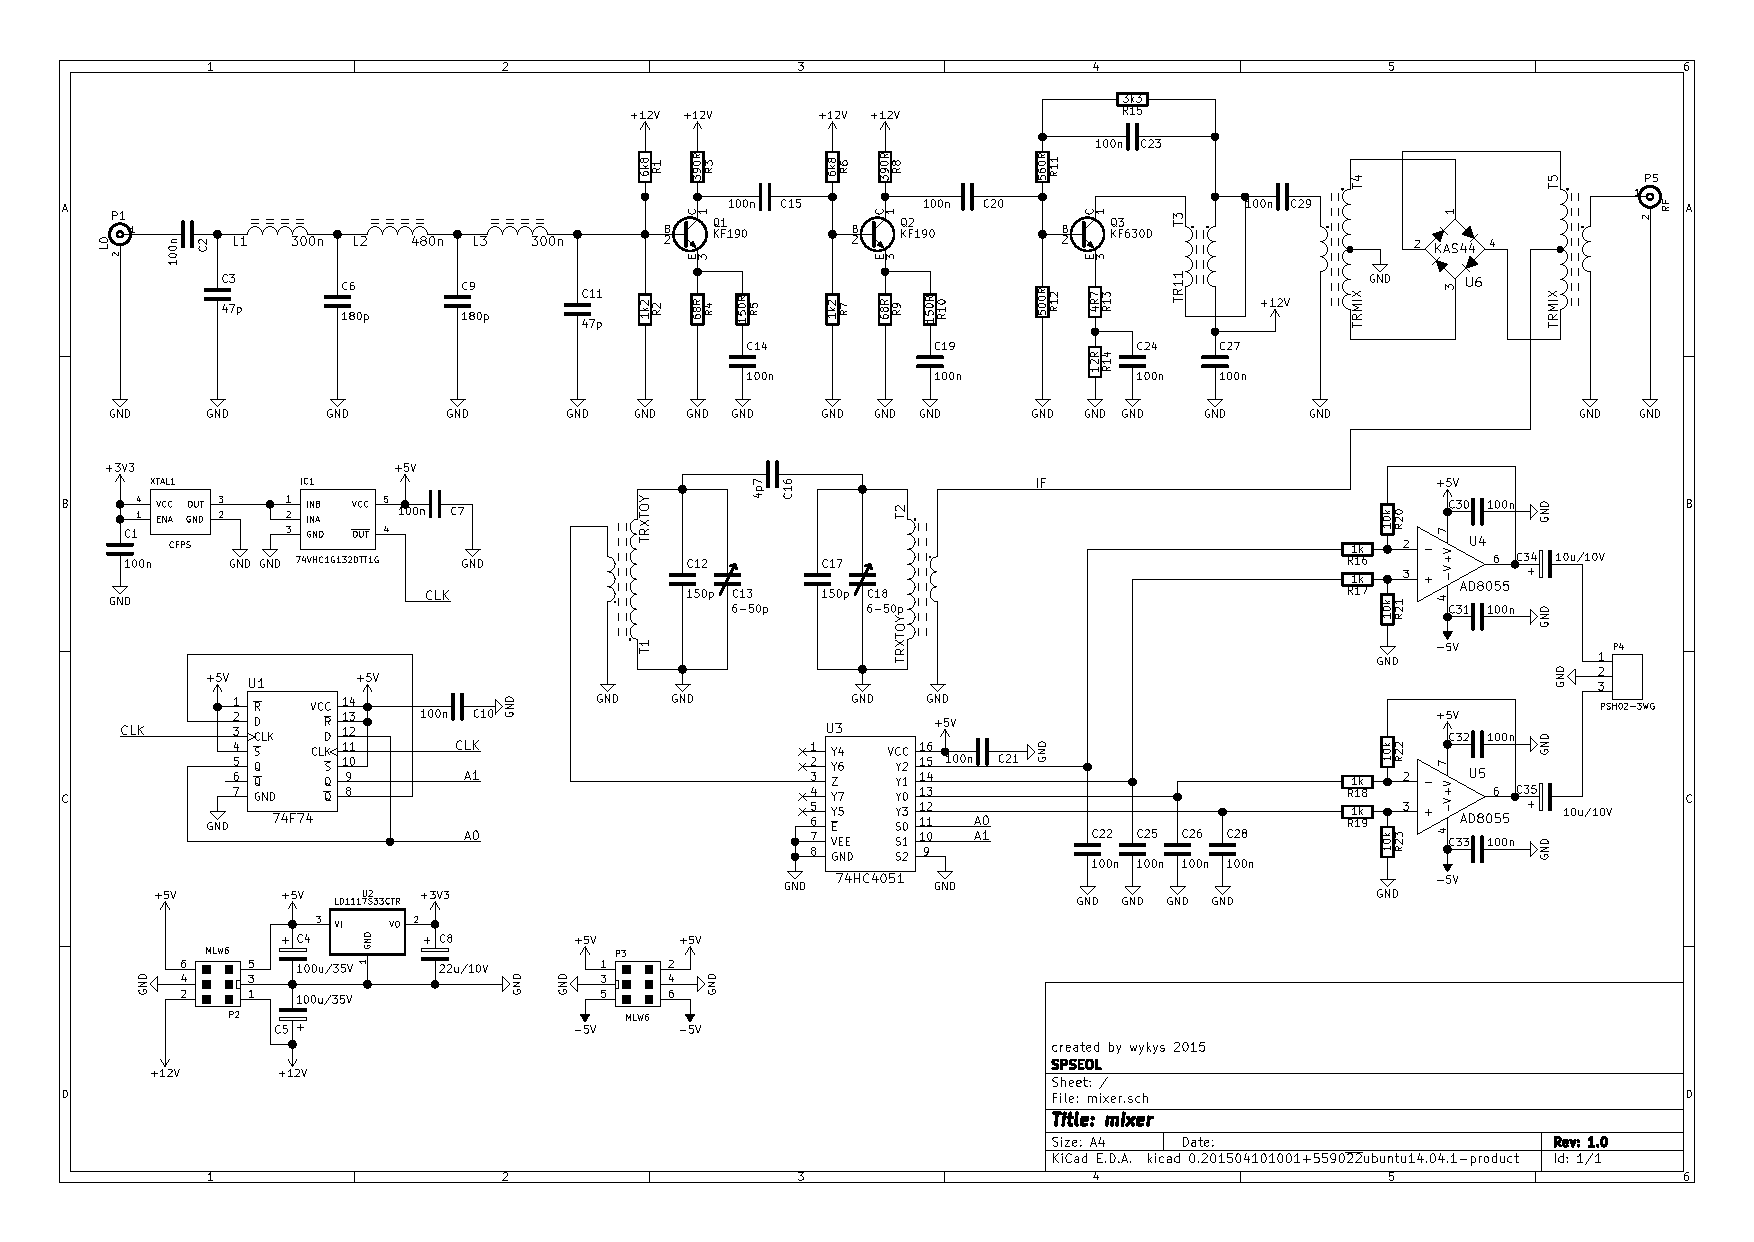
\includepdf[landscape=true]{img/mix/sch.pdf}

% DPS
\begin{figure}[H]
	\centering
	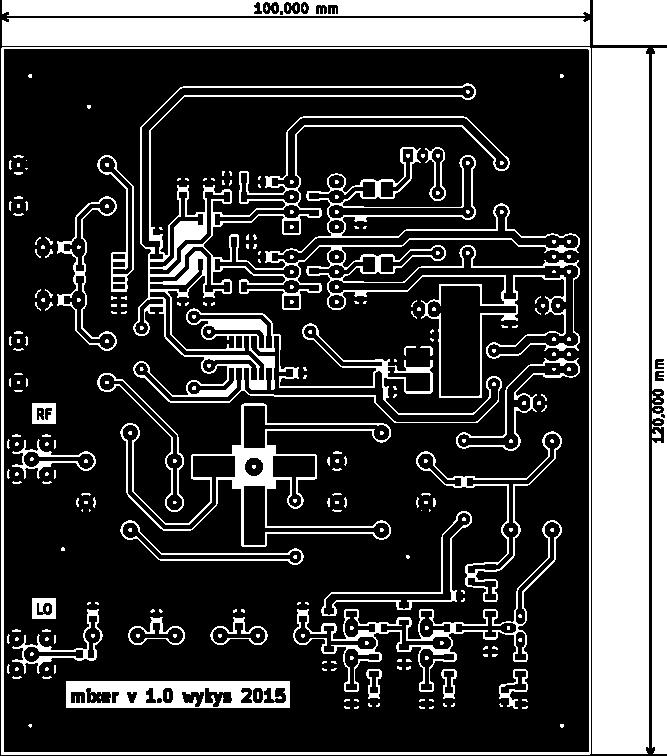
\includegraphics[width=170mm]{img/mix/cu_b.pdf}
	\caption{Deska plošného spoje vrstva mědi}    		
\end{figure}

% os f
\begin{figure}[H]
	\centering
	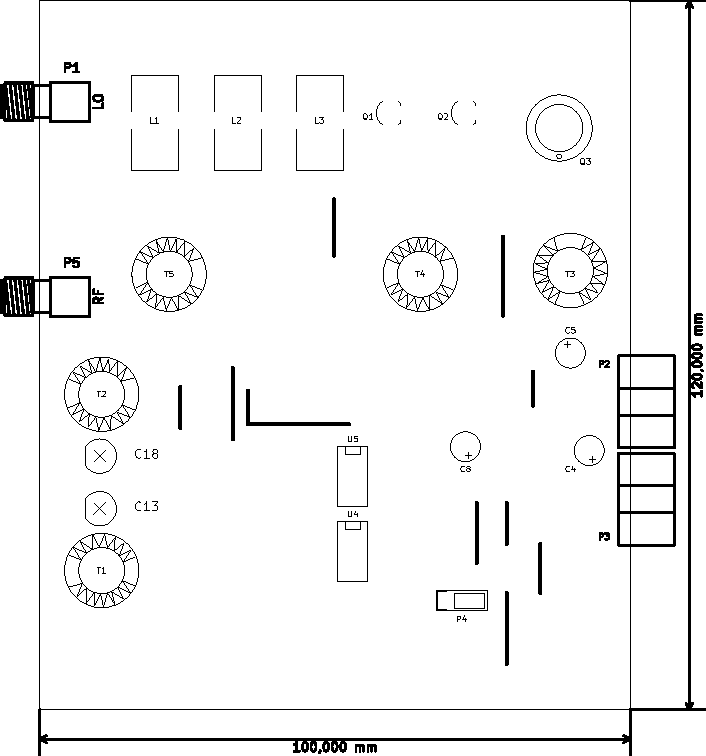
\includegraphics[width=170mm]{img/mix/os_f.pdf}
	\caption{Osazovací plán řídící jednotky, pohled na horní stranu součástek}    		
\end{figure}

% os b
\begin{figure}[H]
	\centering
	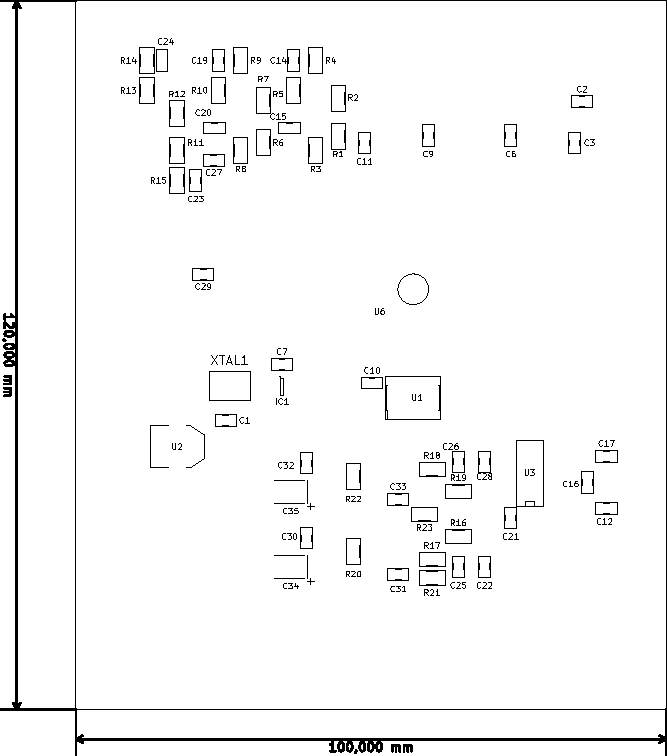
\includegraphics[width=170mm]{img/mix/os_b.pdf}
	\caption{Osazovací plán řídící jednotky, pohled na horní stranu součástek}    		
\end{figure}

\begin{table}[H]
	\begin{center}
		\begin{tabular}[H]{!{\vrule width 1pt}c|c|c|c!{\vrule width 1pt}}
		    \specialrule{1pt}{0pt}{0pt} 
		    \textbf{Určovatel}	&	\textbf{Pouzdro}	&	\textbf{Množství}	&	\textbf{Určení}	\\\specialrule{1pt}{0pt}{0pt} 			
			M1,M2,M3,M4	&	M3	&	5	&	M3	\\\hline
			T1,T2	&	Amidon-T-44-2	&	2	&	TRXTOY	\\\hline
			T5,T4	&	Inductor\_choke	&	2	&	TRMIX	\\\hline
			T3	&	N5	&	1	&	TR11	\\\hline
			C1,C2,C7,C10	&	C\_0805	&	4	&	100n	\\\hline
			C14,C15,C19-C33	&	C\_0805	&	17	&	100n	\\\hline
			C3,C11	&	C\_0805	&	2	&	47p	\\\hline
			C4,C5	&	Elko\_vert\_11x5mm\_RM2.5	&	2	&	100u/35V	\\\hline
			C6,C9	&	C\_0805	&	2	&	180p	\\\hline
			C8	&	Elko\_vert\_11x5mm\_RM2.5	&	1	&	22u/10V	\\\hline
			C12,C17	&	C\_0805	&	2	&	150p	\\\hline
			C13,C18	&	CT	&	2	&	6-50p	\\\hline
			C16	&	C\_0805	&	1	&	4p7	\\\hline
			C34,C35	&	Tantal\_Size\_B	&	2	&	10u/10V	\\\hline
			IC1	&	SOT-23-5	&	1	&	74VHC1G132DTT1G	\\\hline
			L1,L3	&	Amidon-T44-2	&	2	&	300n	\\\hline
			L2	&	Amidon-T-44-2	&	1	&	480n	\\\hline
			P1	&	MCX	&	1	&	LO	\\\hline
			P2,P3	&	vasch\_strip\_3x2\_90	&	2	&	MLW6	\\\hline
			P4	&	Socket\_Strip\_Straight\_1x03	&	1	&	PSH02-3WG	\\\hline
			P5	&	MCX	&	1	&	RF	\\\hline
			Q3	&	TO5	&	1	&	KF630D	\\\hline
			R1,R6	&	R\_1206	&	2	&	6k8	\\\hline
			R2,R7	&	R\_1206	&	2	&	1k2	\\\hline
			R3,R8	&	R\_1206	&	2	&	390R	\\\hline
			R4,R9	&	R\_1206	&	2	&	68R	\\\hline
			R5,R10	&	R\_1206	&	2	&	150R	\\\hline
			R11	&	R\_1206	&	1	&	560R	\\\hline
			R12	&	R\_1206	&	1	&	500R	\\\hline
			R13	&	R\_1206	&	1	&	4R7	\\\hline
			R14	&	R\_1206	&	1	&	12R	\\\hline
			R15	&	R\_1206	&	1	&	3k3	\\\hline
			R16,R17,R18,R19	&	R\_1206	&	4	&	1k	\\\hline
			R20,R21,R22,R23	&	R\_1206	&	4	&	10k	\\\hline
			U1	&	SOIC-14	&	1	&	74F74	\\\hline
			U2	&	SOT-223	&	1	&	LD1117S33CTR	\\\hline
			U3	&	SO-16-N	&	1	&	74HC4051	\\\hline
			U4,U5	&	DIP-8	&	2	&	AD8055	\\\hline
			U6	&	M234\_NoHole\_Housing	&	1	&	KAS44	\\\hline
			XTAL1	&	SMD7x5	&	1	&	CFPS	\\\hline
			Q2,Q1	&	TO-92\_Rugged\_Reverse	&	2	&	KF190 \\\specialrule{1pt}{0pt}{0pt} 
		\end{tabular}

		\caption{Tabulka použitých součástek pro desku DDS, ostatní zde nebyli uvedeny z důvodu nedostatku papíru}
		\label{tab:s1}      
	\end{center}
\end{table}


	\section{Zdroj napětí}
\indent\indent Pro napájení jednotlivých bloků je potřeba zajistit tři napětí a to o hodnotě $+5~V$, $-5~V$ a $+12~V$. Toto zabezpečuje zdroj realizovaný pomocí dvou transformátoru  TR1 a TR2.

Transformátor TR1 má symetrické vinutí, které je zapojeno do série. Krajní vývody těchto vinutí jsou připojeny na dvoucestný usměrňovač realizovaný Graetzovým můstkem . Filtrační kondenzátory jsou pak připojeny z kladného a záporného pólu usměrňovače proti střednímu vodiči, který vznikl spojením vinuti transformátoru. Z takto připraveného symetrického napětí jsou pak napájeny integrované stabilizátory 7805 a 7905, na jejichž výstupech jsou stabilizovaná napětí $\pm5~V$.

Zdroj $+12~V$ je tvořen transformátorem TR2 Graetzovým můstkem D1, filtračním kondenzátorem C3 a stabilizátorem 7812 (U3). Pro ochranu stabilizátoru je použito přemostění diodami D3, D4 a D5.

% schéma
\begin{landscape}
	\begin{figure}[h]
		\centering 	
		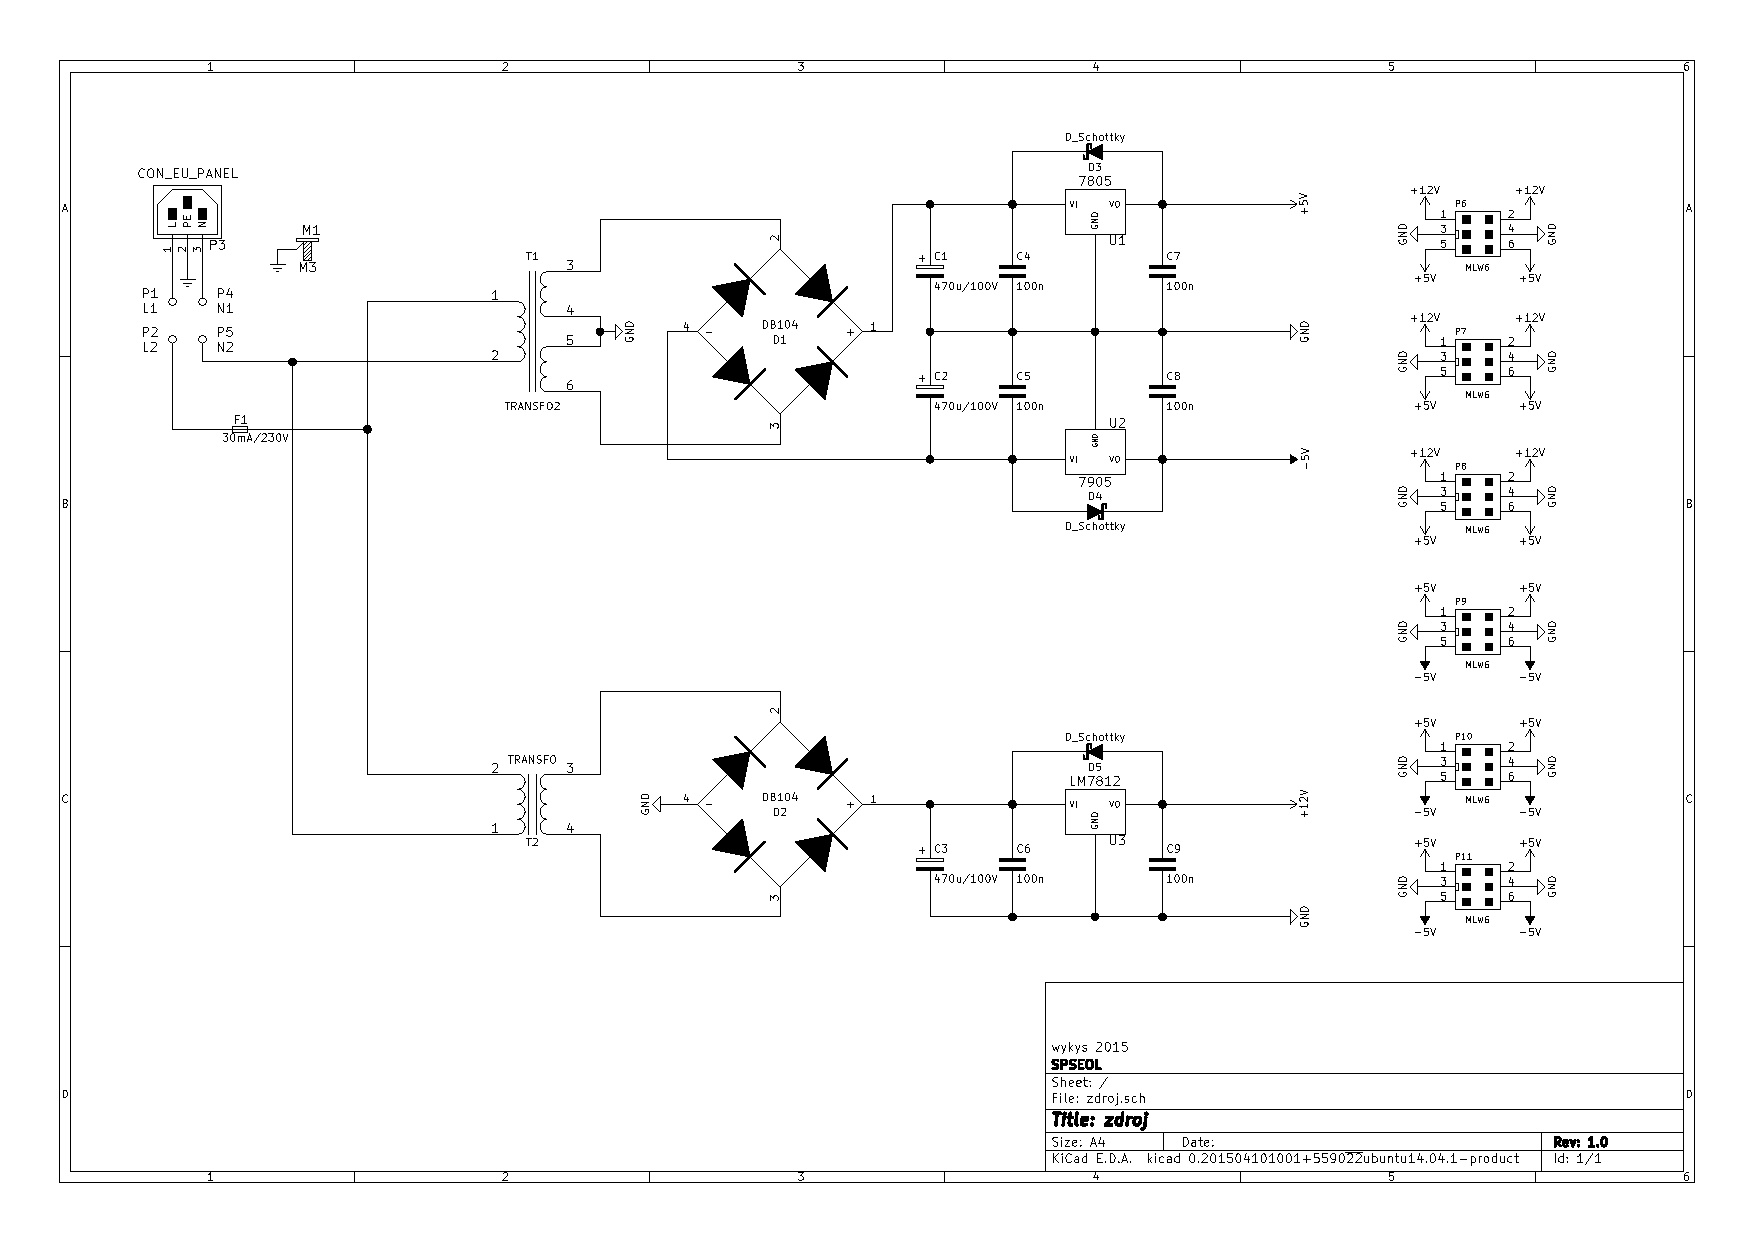
\includegraphics[height=\textwidth]{img/zdroj/sch.pdf}
		\caption{Schéma zapojení zdroje napětí}	
	\end{figure}
\end{landscape}
%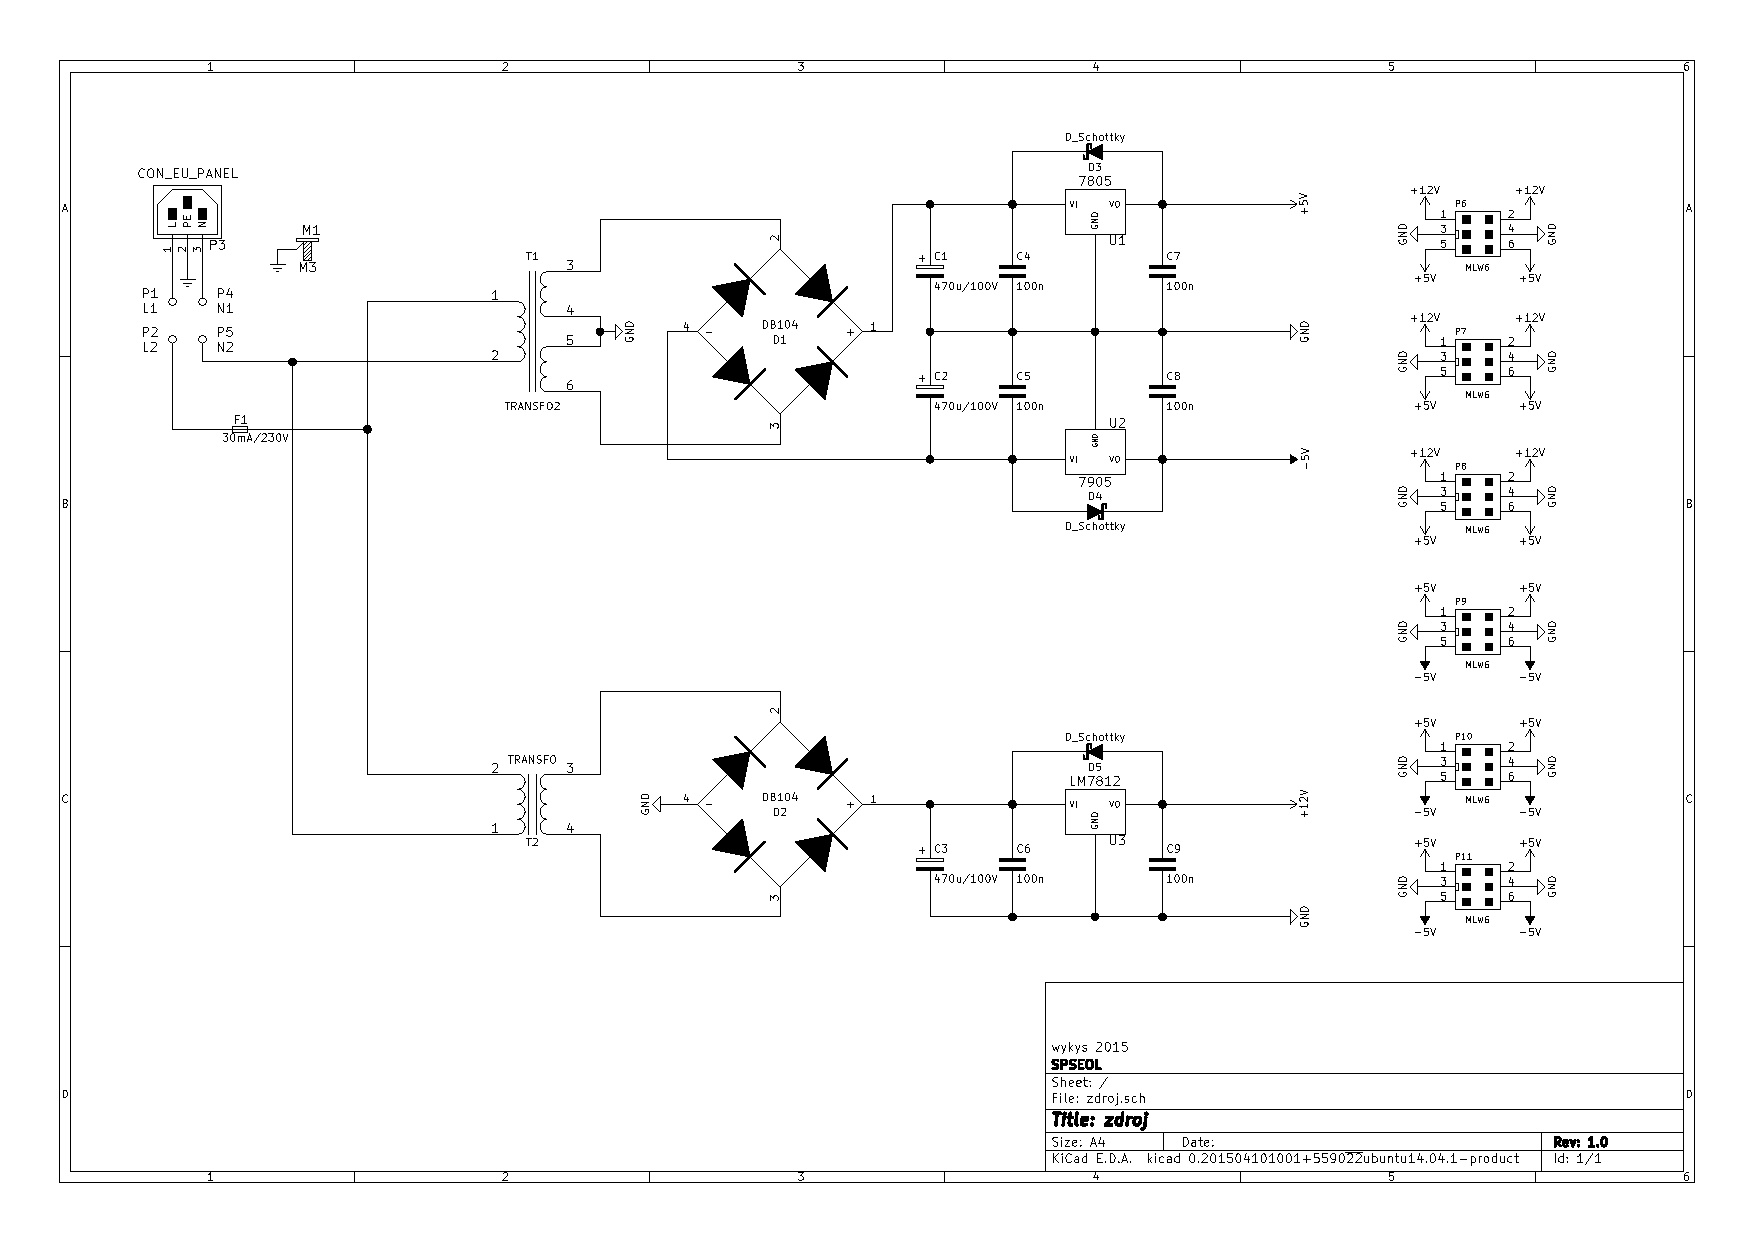
\includepdf[landscape=true]{img/zdroj/sch.pdf}

% DPS
\begin{figure}[H]
	\centering
	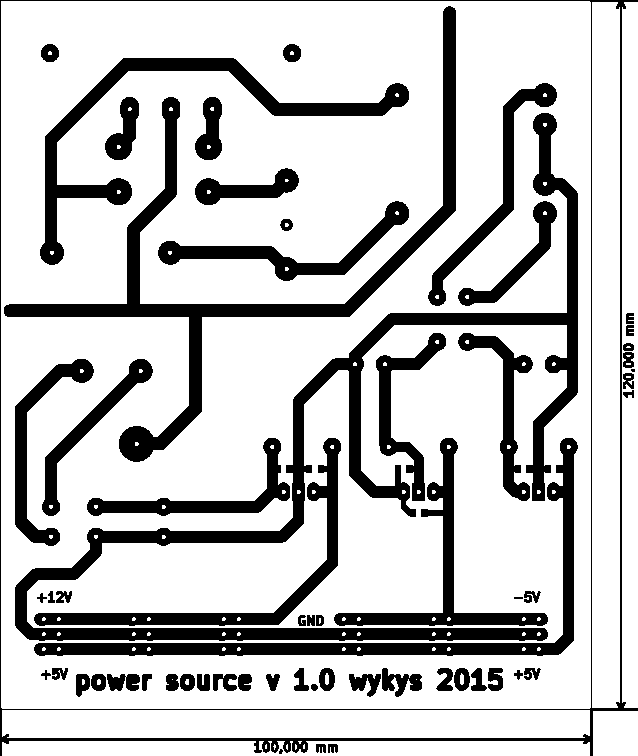
\includegraphics[width=170mm]{img/zdroj/cu_b.pdf}
	\caption{Deska plošného spoje zdroje napětí vrstva mědi}    		
\end{figure}

% os f
\begin{figure}[H]
	\centering
	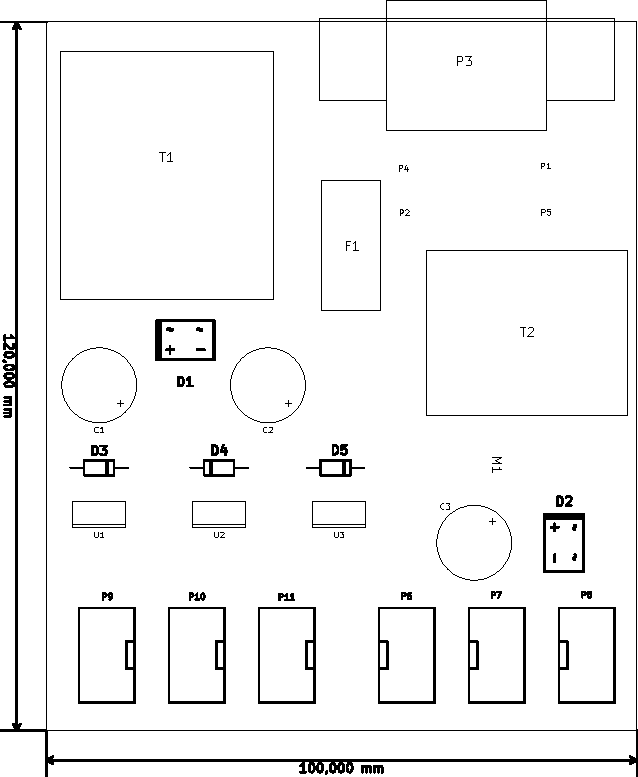
\includegraphics[width=170mm]{img/zdroj/os_f.pdf}
	\caption{Osazovací plán zdroje napětí, pohled na horní stranu součástek}    		
\end{figure}

% os b
\begin{figure}[H]
	\centering
	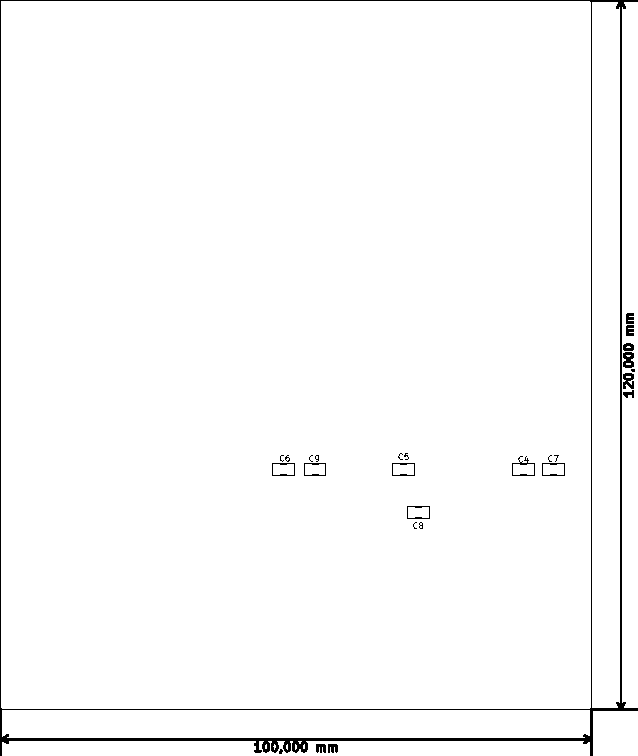
\includegraphics[width=170mm]{img/zdroj/os_b.pdf}
	\caption{Osazovací plán zdroje napětí, pohled na horní stranu součástek}    		
\end{figure}

\begin{table}[H]
	\begin{center}
		\begin{tabular}[H]{!{\vrule width 1pt}c|c|c|c!{\vrule width 1pt}}
		    \specialrule{1pt}{0pt}{0pt} 
		    \textbf{Určovatel}	&	\textbf{Pouzdro}	&	\textbf{Množství}	&	\textbf{Určení}	\\\specialrule{1pt}{0pt}{0pt} 						
			C1,C2,C3	&	Elko\_vert\_25x12.5mm\_RM5	&	3	&	470u/100V	\\\hline
			C4-C9	&	C\_0805	&	6	&	100n	\\\hline
			D1,D2	&	bridge\_DFM	&	2	&	DB104	\\\hline
			D3,D4,D5	&	diode\_do41	&	3	&	D\_Schottky	\\\hline
			F1	&	fuse\_socket	&	1	&	32mA/230V	\\\hline
			M1	&	M3	&	1	&	M3	\\\hline
			P1	&	SolderWirePad\_single\_2mmDrill	&	1	&	L1	\\\hline
			P2	&	SolderWirePad\_single\_2mmDrill	&	1	&	L2	\\\hline
			P4	&	SolderWirePad\_single\_2mmDrill	&	1	&	N1	\\\hline
			P5	&	SolderWirePad\_single\_2mmDrill	&	1	&	N2	\\\hline
			P6-P11	&	vasch\_strip\_3x2	&	6	&	MLW6	\\\hline
			T1	&	BV\_EI\_382	&	1	&	TRANSFO2	\\\hline
			T2	&	BV\_EI\_303	&	1	&	TRANSFO	\\\hline
			U1	&	LM78XXV	&	1	&	7805	\\\hline
			U2	&	LM79XXV	&	1	&	7905	\\\hline
			U3	&	LM78XXV	&	1	&	LM7812	\\\hline
			P3	&	CON\_EU\_PANEL	&	1	&	CON\_EU\_PANEL	\\\specialrule{1pt}{0pt}{0pt} 
		\end{tabular}

		\caption{Tabulka použitých součástek pro desku zdroje}
		\label{tab:s1}      
	\end{center}
\end{table}

	\clearpage
\section{Softwarové zpracování}
\indent\indent Signály převedené do nízkofrekvenčního pásma jsou navzorkovány zvukovou kartou a následně v reálném čase zpracovávané programem.
\subsection{Základní princip zpracování}
\indent\indent Program nejprve převede přijímaný signál pomocí diskrétní furierovy transformace do frekvenční oblasti. V tomto okamžiku se generují i data pro zobrazování waterfall. Když jsou data převedena do frekvenční oblasti, tak si vybereme požadované pásmo požadované frekvence. Poté projde signál konvolučním filtrem, který provede vybranou demodulaci. Nakonec se přijímaný signál převede zpátky do časové oblasti pomocí diskrétní inverzní furierovy transformace. V posledním kroku signál projde filtry pro zbavení stejnosměrné složky, která vzniká při vzorkování, signál projde ještě dolní propustí a je možné jej dostat ze zvukové karty ven pomocí linkového výstupu.

% telegrafie
\begin{figure}[H]
	\centering
	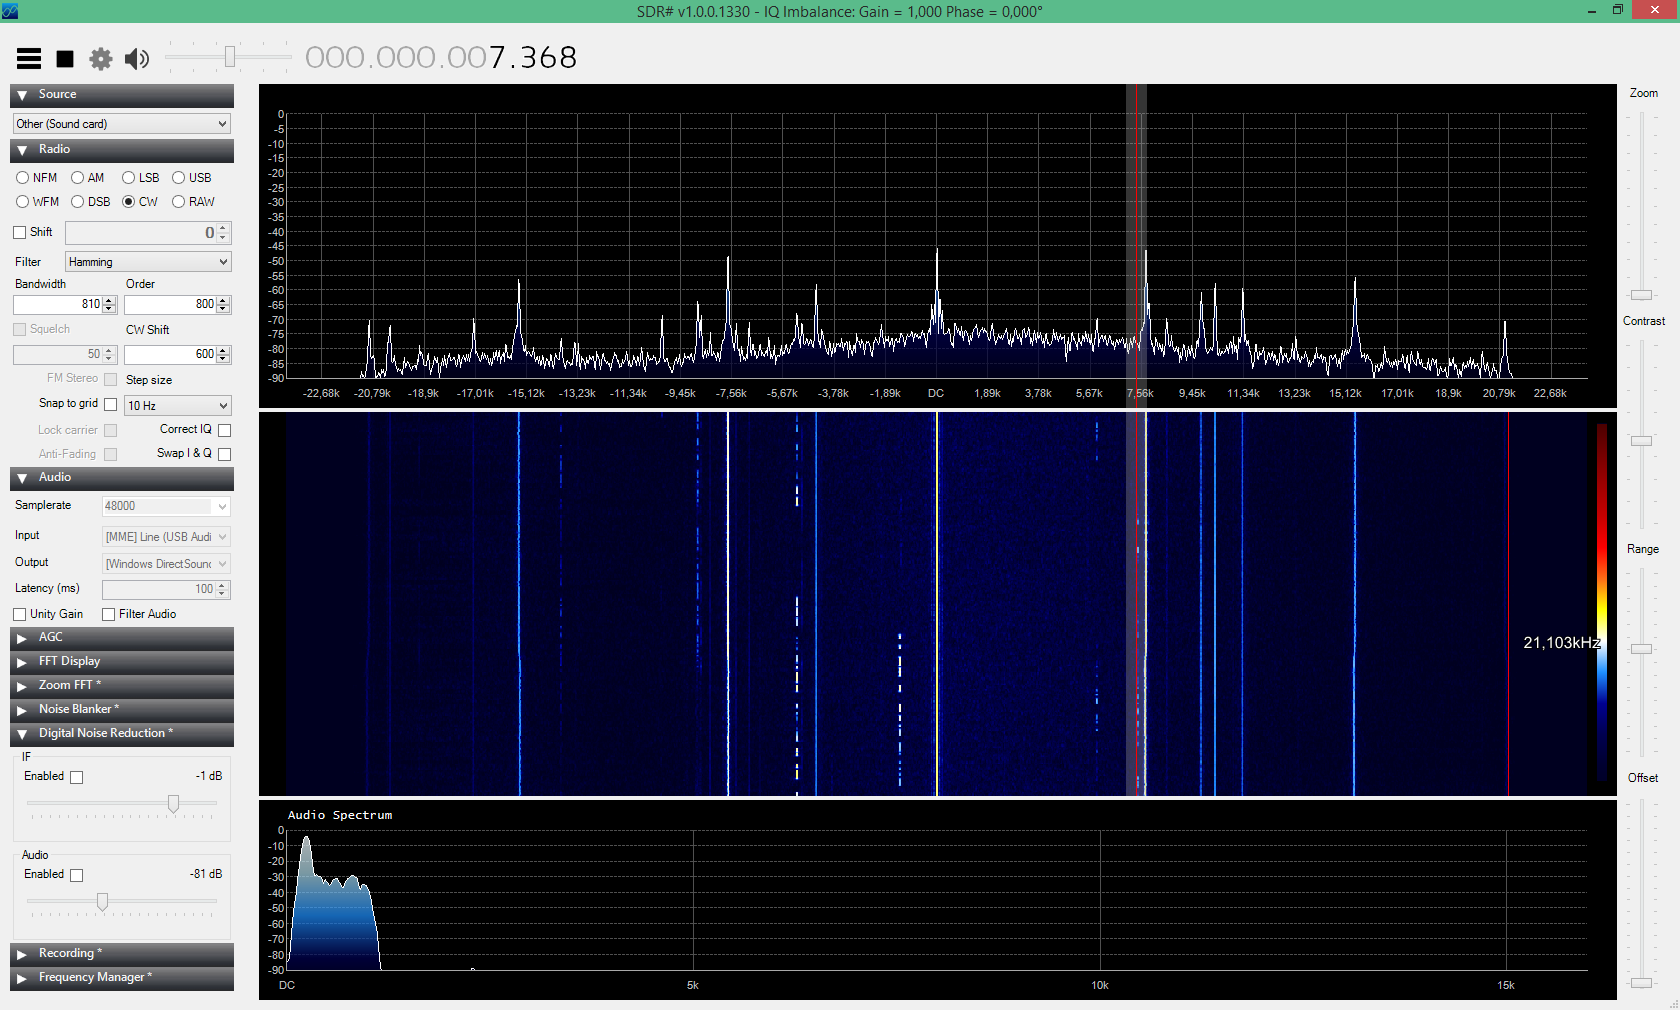
\includegraphics[width=170mm]{img/prijem.png}
	\caption{Ukázka příjmu telegrafie na kmitočtu $14.01~MHz$}    		
\end{figure}

\subsection{Sharp SDR}
\indent\indent Ke zpracovávání signálu jsem si vybral program Sharp SDR. Tento program umožňuje zpracování signálů I a Q ze zvukové karty. Jeho velkou předností je snadné ovládání. Můžeme si zde měnit šířku přijímaného pásma, dokáže demodulavat jak AM modulace, tak také modulace FM. Demodulování CW je samozřejmostí. Dále je možné nastavovat potlačení šumu ve výstupním i vstupním signálu.
	\clearpage

\section{Návod k obsluze zařízení}
\indent\indent Ovládání zařízení je velice intuitivní. Zařízení stačí připojit kabelem, které má na obou koncích konektor stereo Jack 3,5 samec do SDR přijímače na čelní panel a druhý konec do linkového vstupu zvukové karty. Čím bude mít zvuková karta vyšší vzorkovací frekvenci, tím větší pásmo budeme moci sledovat na osobním počítači s obslužným softwarem. Po připojení kabelu stačí k zařízení zezadu připojit napájecí kabel, jedná se o klasickou ,,euro šňůru''. Poté již jen stačí na  čelním panelu stisknout vypínač a na osobním počítači spustit obslužný software Sharp SDR. Ovládání Software je velmi jednoduché. Vlevo na postranním panelu se nastavují parametry zpracování signálu jako: způsob demodulace, šířka pásma, potlačení stejnosměrné složky, potlačení šumu atd. SDR přijímač se ovládá ještě jednodušeji. Otáčením rotačního enkodéru měníme výstupní frekvenci. Pokud stiskneme enkodér, přepneme se do módu, ve kterém otáčením enkodéru měníme ladící krok. Opětovným stiskem enkodéru se dostaneme zpátky do módu ladění přijímané frekvence.

% os b
\begin{figure}[H]
	\centering
	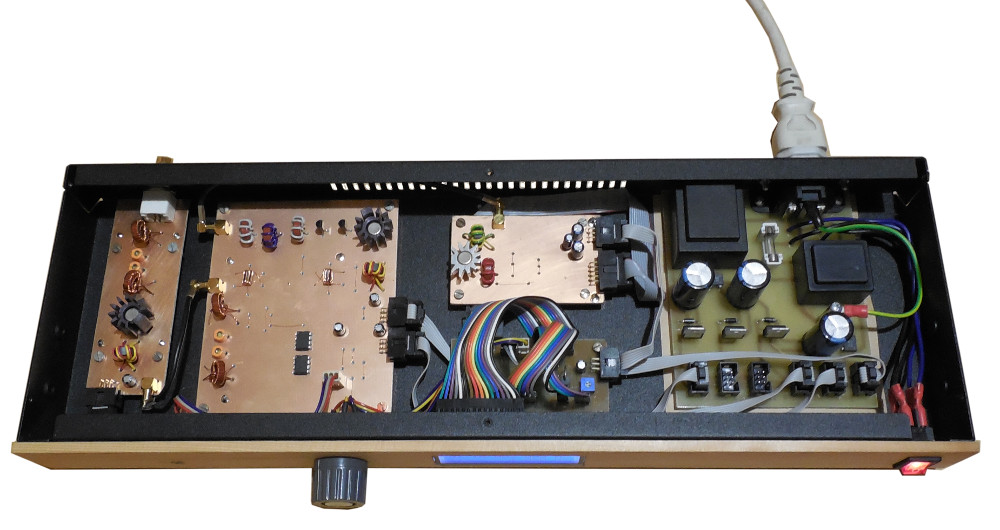
\includegraphics[width=170mm]{img/bez_kritu_sm.jpg}
	\caption{Hotové zařízení bez horní části krabice}    		
\end{figure}

% os b
\begin{figure}[H]
	\centering
	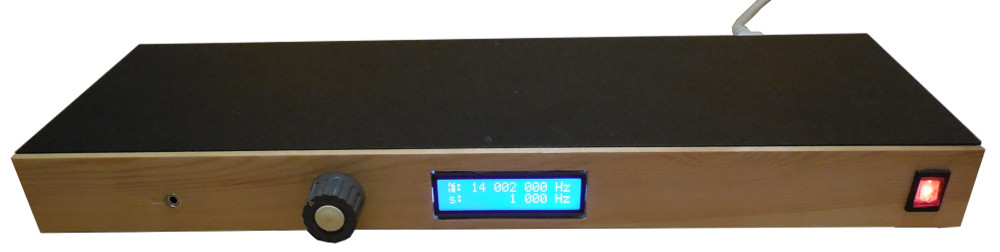
\includegraphics[width=170mm]{img/s_kritem_sm.jpg}
	\caption{Hotové zařízení v kompletní krabici rackových rozměrů}    		
\end{figure}

\clearpage
	\section*{Závěr}
\addcontentsline{toc}{section}{Závěr}
\indent\indent Cílem mé práce bylo vytvořit SDR přijímač pro KV pásmo. To se mi nakonec povedlo, i když musím uznat že cesta k cíli nebyla vůbec jednoduchá. Přijímač je určený pro příjem radioamatérského pásma $20~m$. Většinu času jsem strávil studiem níže uvedených materiálů, protože tohle je můj první přijímač. O to větší z něj mám ale radost. Přijímači jsem změřil selektivitu vstupního napětí, aby se ověřil vstupní aktivní filtr popsaný ve druhé kapitole. Výsledky měření jsou shrnuty v obrázku číslo 3. Během vývoje byly největší problémy s návrhem pásmových propustí, vystřídal jsem velké množství železo-prachových a feritových jared, tvarů a zapojení, než jsem došek k filtrům uvedeným v této práci. Další komplikací při vývoji byl směšovač navinutý na toroidech z materiálu Amidon T-44-2. Tyto toroidy měly totiž moc malé $A_L$, díky čemuž na nich namotané cívky měly na $14~MHz$ moc malou reaktanci. Konkrétně $22~\Omega$. Nakonec se osvědčily obyčejné tlumivky z železo-prachových jader, které měly reaktanci na $14~MHz$ několik set ohmů. Když byly tyto problémy překonány, tak bylo třeba navrhnout plošné spoje. Na těchto plošných spojích se zařízení ale chovalo jinak a tak bylo nutné poupravit hodnoty kondenzátorů jinak než byly na prototypech. Na finálních verzích plošných spojů se filtry chovají mnohem ostřeji než na testovacích destičkách. to je způsobeno zkrácením všech cest na minimum, které jednostranné plošné spoje umožní. Zařízení jsem nakonec s tátovou pomocí zapouzdřil do rackové krabice.

Na řídící destičce je nachystaný konektor pro USART, už mám nachystaný i další modul pro převod USART na USB, díky němuž bude v blízké době možné zařízení kompletně ovládat z osobního počítače. To by umožnilo se vhodným software použít toto zařízení jako maják. Tento maják by fungoval následovně. Pomocí internetu by se připojil operátor vzdálené radio stanice k uživatelskému rozhraní pro obsluhu. Pomocí svého vysílače by vyslal například svůj volací znak. Pokud by byla radiostanice v dosahu, tak by mu aplikace přehrála audio záznam příjmu, tak jak jde slyšet v mém přijímači. Díky tomu by si mohl uživatel vzdálené radiostanice udělat obrázek o tom, jaký má jeho vysílač dosah.	
	\clearpage
\def\refname{Seznam použité literatury a studijních materiálů}
\begin{thebibliography}{10}

	\bibitem[1]{nitro}
	{\em  Karel OK2ZI:}
		{\bf Širokopásmový vf zesilovač $[$\textmd{online}$]$ $[$\textmd{cit. 11-4-2015}$]$}\\
		Dostupné z: \texttt{\href{http://ok2zi.blogspot.cz/2010/11/pasmova-propust-predzesilovac-pro-160m.html}{http://ok2zi.blogspot.cz\\/2010/11/pasmova-propust-predzesilovac-pro-160m.html}}
		
	\bibitem[2]{OK1UNL}
	{\em Doc. OK1UNL:}
		{\bf Úvod do SDR $[$\textmd{online}$]$ $[$\textmd{cit. 13-4-2015}$]$}\\
		Dostupné z: \texttt{\url{http://www.ok1cjb.cz/index.php}}
		
	\bibitem[3]{frekvenční spektrum na výstupu DDS}
	{\em Analog Devices:}
		{\bf Podpora pro vývojáře DDS generátorů$[$\textmd{online}$]$ $[$\textmd{cit. 13-4-2015}$]$}\\
		Dostupné z: \texttt{\url{http://www.analog.com/designtools/en/simdds/dtDDSMain.aspx}}
		
	\bibitem[4]{s.maslan@seznam.cz}
	{\em Vlastimil Slinták:}
		{\bf FFT na AVR $[$\textmd{online}$]$ $[$\textmd{cit. 13-4-2015}$]$}\\
		Dostupné z: \texttt{\url{http://elektronika.kvalitne.cz/\\ATMEL/necoteorie/transformation/AVRFFT/AVRFFT.html}}
		
	\bibitem[5]{Mikael Q Kuisma}
	{\em Mikael Q Kuisma:}
		{\bf Zpracování I a Q signálů $[$\textmd{online}$]$ \\$[$\textmd{cit. 13-4-2015}$]$}\\
		Dostupné z: \texttt{\url{http://whiteboard.ping.se/SDR/IQ}}


\bibitem[6]{Jarda OK1HDU}
	{\em Jarda OK1HDU:}
		{\bf Úvod do radioelektroniky $[$\textmd{online}$]$ \\$[$\textmd{cit. 13-4-2015}$]$}\\
		Dostupné z: \texttt{\url{http://599.cz/search.php?\\rsvelikost=sab\&rstext=all-phpRS-all\&rstema=13\&stromhlmenu=13}}


\bibitem[7]{OK2IP}
	{\em OK2IP:}
		{\bf web zabývající se problematikou SDR $[$\textmd{online}$]$ \\$[$\textmd{cit. 13-4-2015}$]$}\\
		Dostupné z: \texttt{\url{http://sdr.ipip.cz/}}


\bibitem[8]{komunitní projekt}
	{\em komunitní projekt:}
		{\bf knihovny určené ke zpracování signálu $[$\textmd{online}$]$ \\$[$\textmd{cit. 13-4-2015}$]$}\\
		Dostupné z: \texttt{\url{http://gnuradio.org/redmine/projects/gnuradio/wiki}}


\bibitem[9]{komunitní projekt}
	{\em komunitní projekt:}
		{\bf software pro zpracování signálu $[$\textmd{online}$]$ \\$[$\textmd{cit. 13-4-2015}$]$}\\
		Dostupné z: \texttt{\url{http://sdrsharp.com/}}


\addcontentsline{toc}{section}{Seznam použité literatury a studijních materiálů} 
\end{thebibliography}

\clearpage
	\listoftables
	\addcontentsline{toc}{section}{Seznam tabulek} 
	\listoffigures	
	\addcontentsline{toc}{section}{Seznam obrázků} 
	\clearpage
\appendix
\section{PŘÍLOHA}
	\subsection{Obsah přiloženého DVD}
	
	\begin{itemize}
		\item Fotodokumentaci zařízení
		\item Fotodokumentaci z vývoje zařízení
		\item Plošné spoje
		\item Demodulační software
		\item Video nahrávky příjmu zde popisovaného zařízení
	\end{itemize}
	

	\label{konec}
\end{document}